\documentclass[book.tex]{subfiles}
\begin{document}
To study the IBM PC it is easier to break it down in small parts. Five sub-systems stand out: Inputs, CPU, RAM, Video, and Audio, together forming a pipeline.\\
\begin{figure}[H]
\centering
\includegraphics[width=\textwidth]{imgs/drawings/fun_pipeline.pdf}
\caption{Hardware pipeline.}
\label{fig:digraph}
\end{figure}

Overall, the pipeline generates a lot of friction since manufacturers had not embraced the gaming industry yet. Some parts are bad, some are very bad, and some were downright impossible to deal with.\\
\par

\begin{figure}[H]
\centering
\begin{tabularx}{\textwidth}{ X X  }
  \toprule
  \textbf{Stage} & \textbf{Quality} \\ \bottomrule
  RAM & Bearable \\ 
  Video & Impossible \\ 
  Audio & Very Poor \\ 
  Inputs & Ok \\ 
  CPU & Impossible \\ \bottomrule
\end{tabularx}
\caption{Component quality for a 3D game engine.}
\end{figure}



\section{CPU: Central Processing Unit}
  
  In 1991 there were 56 millions PCs in USA \footnote{"Computers". Collier's Encyclopedia. Vol. 7, 1992: 114, 129.}. The performances of these machines were so overwhelmingly dominated by the CPU that a PC was referred to not by its brand or GPU\footnote{There was no GPU yet. The term was coined by Nvidia in 1999, who marketed the GeForce 256 as "the world's first GPU", or Graphics Processing Unit.} but by the main chip inside. If a PC had a 80386 or equivalent, it was called a "386". If it had an Intel 80286, it was a "286".\\
\subsection{Overview}
  The ubiquitous CPU manufacturer was Intel with its line of x86 microprocessors. Machines based on the 16 bits 80286 processor did not sell well\footnote{Bill Gates dubbed it "Brain Dead"} but its successor the 80386 introduced in 1985 was immensely successful\footnote{SALES}. As a result, Wolfenstein 3D was designed to run on a PC with a 386 CPU, with degraded performance (yet still playable) on a 286.\\
\par


\begin{figure}[H]
\centering
  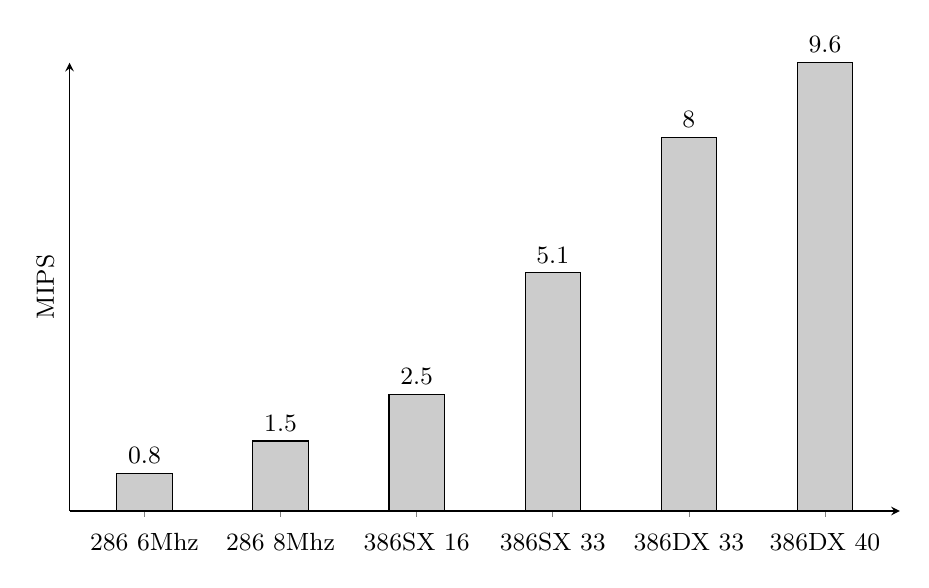
\begin{tikzpicture}[font=\small]
    \begin{axis}[
      width=1.0\textwidth,
      height=0.6\textwidth,
      ybar,
      bar width=20pt,
      ylabel={MIPS},
      ymin=0,
      ytick=\empty,
      xtick=data,
      axis x line=bottom,
      axis y line=left,
      enlarge x limits=0.11,
      symbolic x coords={286 6Mhz,286 8Mhz,386SX 16,386SX 33,386DX 33,386DX 40},
      xticklabel style={anchor=base,yshift=-\baselineskip},
      nodes near coords={\pgfmathprintnumber\pgfplotspointmeta}
    ]
      \addplot[fill=black!20,draw=black] coordinates {
        (286 6Mhz,0.8)
        (286 8Mhz,1.5)
        (386SX 16,2.5)
        (386SX 33,5.1)
        (386DX 33,8)
        (386DX 40,9.6)
      };
    \end{axis}
   
   \end{tikzpicture}
   \caption{Comparison\protect\footnotemark of CPUs with MIPS \protect\footnotemark.}
 \end{figure}
 \footnotetext{Source: "Roy Longbottom's PC Benchmark Collection: http://www.roylongbottom.org.uk/mips.htm\#anchorIntel2".}
 \footnotetext{Million Instructions Per Second.}
 \par
  \textbf{\underline{Trivia :}} A modern processor such as the Intel Core i7 3.33 GHz operates at close to 180,000 MIPS.\\
  \par
 Intel built two versions of the 386: The 386-SX and 386-DX. They are identical processors yet the DX version is almost twice as powerful as the SX (on the chart the \cw{386 SX 33Mhz} and the \cw{386 DX 33Mhz} are respectively at 5.1 and 8 MIPS). This is due to a data bus between the CPU and the RAM being twice as wide on the DX (32 bits vs 16 bits). Despite its inferiority, the SX sold well because it was cheaper and a lot of people had no idea what a "bus" was, they just wanted "a 386".\\



 \par
\textbf{\underline{Trivia :}} Two other companies produced Intel clones: AMD and Cyrix. Their mediocre performances did not justify the lower cost and as a result they never gained significant market share. Almost all PCs featured an Intel CPU. Interestingly, AMD evolved to become a serious challenger\footnote{The history of AMD vs Intel litigations could be the subject of a book.} while Cyrix merged with National Semiconductor in 1997.\\
\par

\subsection{The Intel 80386}
The trip from blueprint to silicon was not a pleasure cruise for the 80386. It started as a side project for a small team in San Jose while select employees in Portland worked on the flagshit P7\footnote{a.k.a Intel i960.}, a CPU using a new instruction set capable of running high level language and memory garbage collection in hardware. When the Portland team hit a wall due to performances, the 386 went from step child to king\footnote{Intel 386 Microprocessor Design and Development Oral History Panel}. Two choices in the design of the 386 contributed to its success. For one the designers decided to listen to the programmers feedback and dropped the idea to use a new instruction set. As a result the 386 is fully backward compatibility with the 286. They also managed to add a 32 bit operating mode which solves many of the memory addressing issues of the 286.\\
\par
\textbf{\underline{Trivia :}}  The 286 was quite unpopular among both programmers and hardware designers. Bill gates called it "brain dead"\footnote{Dewar, Robert B. K.; Smosna, Matthew (1990). Microprocessors: A Programmer's View. New York: McGraw-Hil} for operating systems and Steve Morris (co-architect of the Intel 8086) called it "Software poison".\\
\par
The 80386 relies on three systems and a three stages instructions pipeline.\\
\par
\begin{figure}[H]
\centering
\includegraphics[width=\textwidth]{imgs/drawings/386_architecture.pdf}
\end{figure}
\par
The Bus Unit is the only difference between a SX and a DX. The SX has a 16 bit bus which allowed PC manufacturers to reuse the design of the 286 motherboards and drove the price down significantly. The DX was had a fully 32 bit Bus unit.
\par
\begin{figure}[H]
\centering
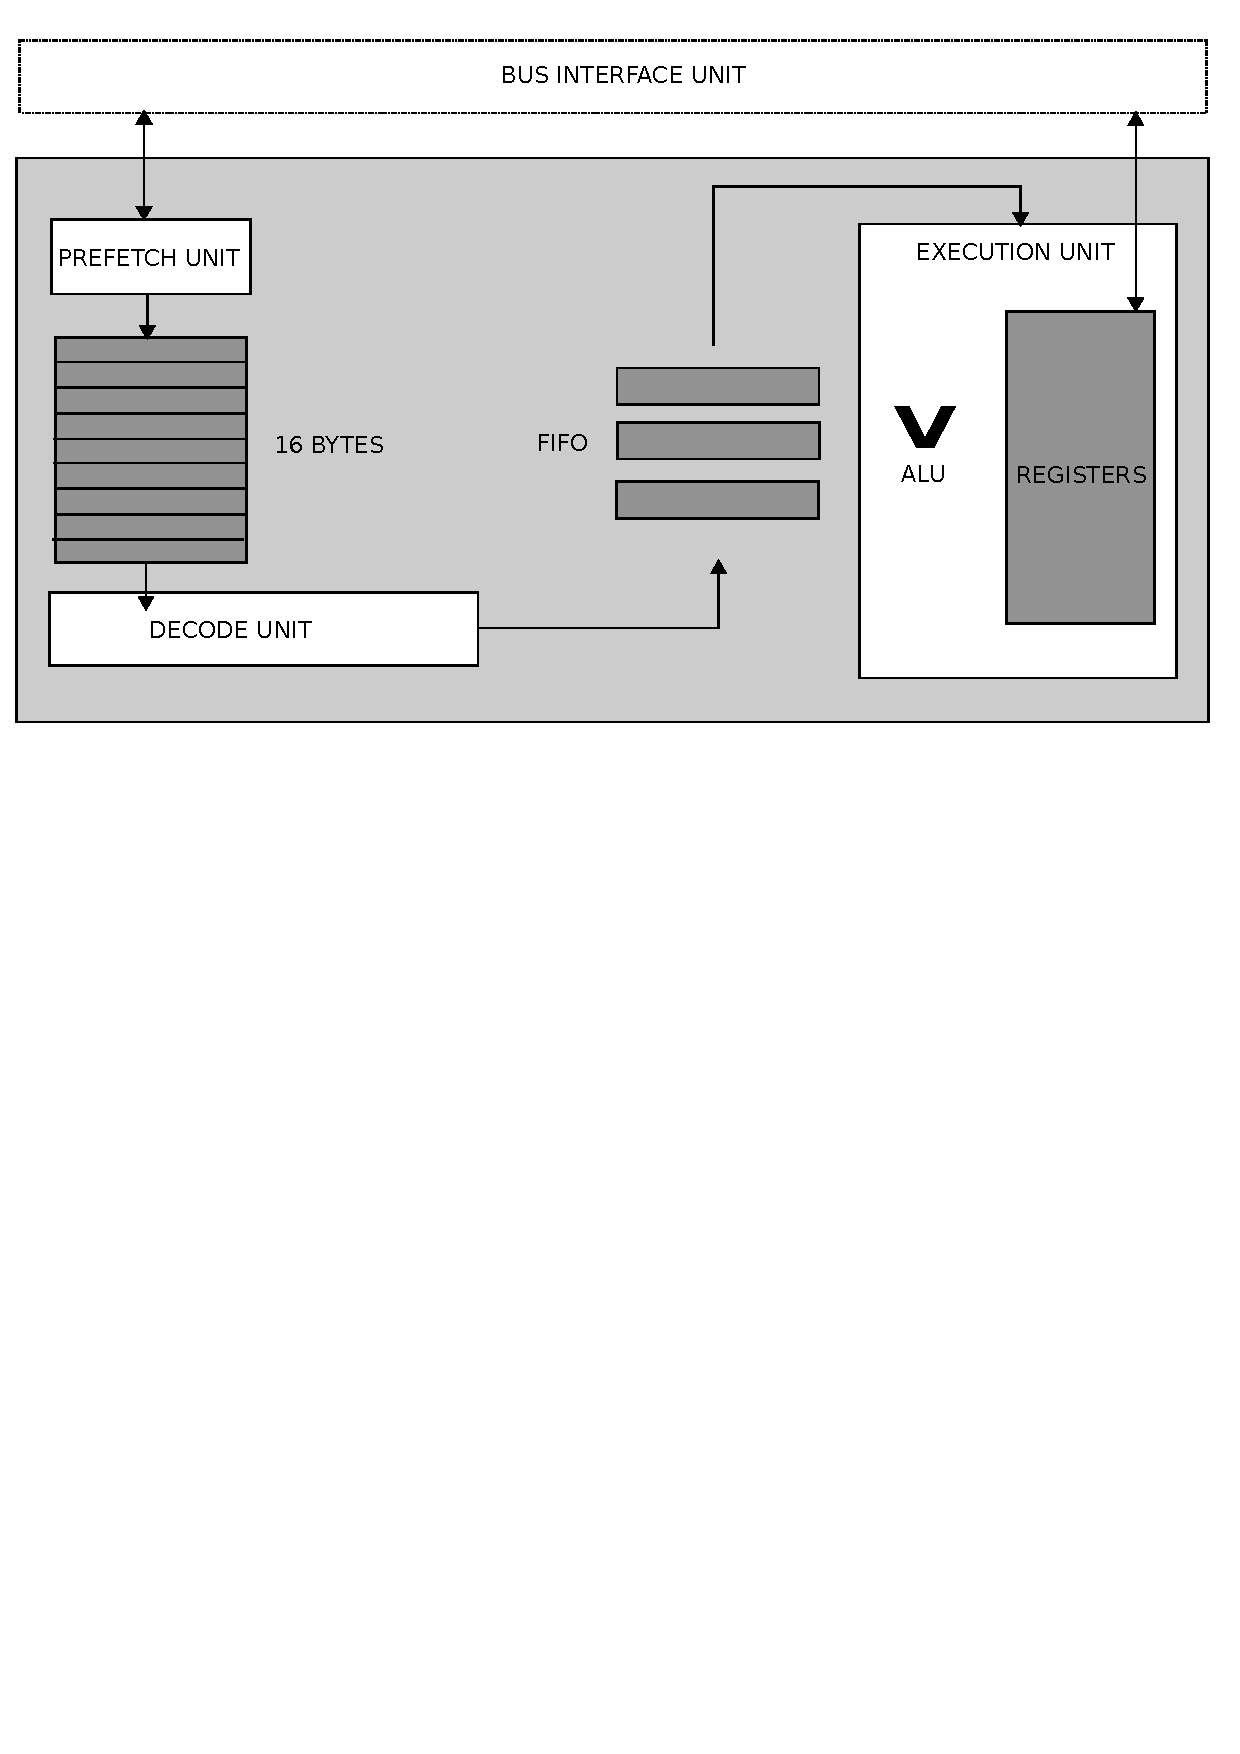
\includegraphics[width=\textwidth]{imgs/drawings/processing_unit.pdf}
\end{figure}
\par
The three units in the execution group form a three stages pipeline: Prefetch, Decode, and Execute. The Prefetch Unit wakes up when the Execution unit is performing but not using the bus and stores instructions in a 16 byte array. The prefetcher is linear and cannot predict the result of a branch. A jump (\cw{JMP}) instruction triggers a flush of the entire pipeline. Instructions go down the pipeline and are decoded by the Decode Unit, the result of the decode operation is storedin a three elements FIFO where they are picked up by the Execution Unit.\\
\par

\begin{figure}[H]
\centering
\includegraphics[width=\textwidth]{imgs/drawings/instruction_pipeline.pdf}\\
\end{figure}
\par
\begin{figure}[H]
\centering
\shadowbox{
  \fullimage{Intel80386.png}
  }
\caption{The Intel 386, 10mmx10mm packing 275,000 transistors}
\end{figure}
\par
From a programming perspective, a 386 CPU can be summarized by the following elements:
\begin{itemize}
\item An Arithmetic Logic Unit performing \cw{add}, \cw{sub}, \cw{mul} et cetera.
\item 15 registers:
\begin{itemize}
  \item 32-bit General Purpose Registers: EAX, EBX, ECX, EDX
  \item 32-bit Index Registers: ESI, EDI, EBP, ESP
  \item 32-bit Program Counter: EIP
  \item 16-bit Segment Registers: CS, DS, ES, FS, GS, SS
  \item 16-bit Status Register
\end{itemize}
\item A 32 bit address bus for up to 4GB of flat addressable RAM
\item Memory Paging Unit
\end{itemize}
 \par
 \textbf{\underline{Trivia :}} Despite its pipeline design, the 386 cannot do an operation in less than two cycles. Even a simple \cw{ADD reg, reg} or \cw{INC reg} take two clocks. This is mostly due to the abscenece of SRAM on-chip cache.\\
 \par
 

  \begin{figure}[H]
\centering  
\begin{tabularx}{\textwidth}{ X  Y }
  \toprule
  \textbf{Instruction type} &  \textbf{Clocks} \\
  \toprule 
   \cw{ADD reg16, reg16} & 2  \\
   \cw{INC reg16} & 2  \\
   \cw{IMUL reg16, reg16} & 12-25\footnote{Not all multiplications are equal. The 80386 uses an early-out multiply algorithm. The actual number of clocks depends on the position of the most significant bit in the optimizing multiplier}  \\
   \cw{IDIV reg16, reg16} & 27 \\
   \cw{MOV [reg16], reg16} & 4 \\
   \cw{OUT [reg16], reg16} & 25 \\
   \cw{IN [reg16], reg16} & 26 \\
  \toprule
\end{tabularx}
\caption{386 instruction cost\protect\footnotemark}
\end{figure}
\footnotetext{Source:INTEL 80386 PROGRAMMER'S REFERENCE MANUAL 1986}





  \subsection{Floating Point}
  
   All that CPU power was not necessarily useful for programming a game. In order to perform the trigonometric computations for 3D effects, the engine has to keep track of the fractional part of each operation. It may not look like an issue since the C programming language has a type (\codeword{float}) precisely for that purpose. But in practice it is a problem, and to understand it we need to understand how that \codeword{float} works.\\
\par
 As David Goldbert famously wrote, \emph{"Floating-point arithmetic is considered an esoteric subject by many people"}\footnote{What every Computer Scientist should know about Floating-Point}. I could not agree more. Yet it is important to understand in order to fully grasp how useful it is to program a 3D engine. In the C language, \codeword{float}s are 32 bits container following the IEEE 754 standard. Their purpose is to store and allow operations on approximation of real numbers. The 32 bits are divided in three sections:\\
\begin{itemize}
  \item One bit S for the sign
  \item Seven bits E for the exponent
  \item Twenty four bits for the mantissa
\end{itemize} 

\begin{figure}[H]
\centering
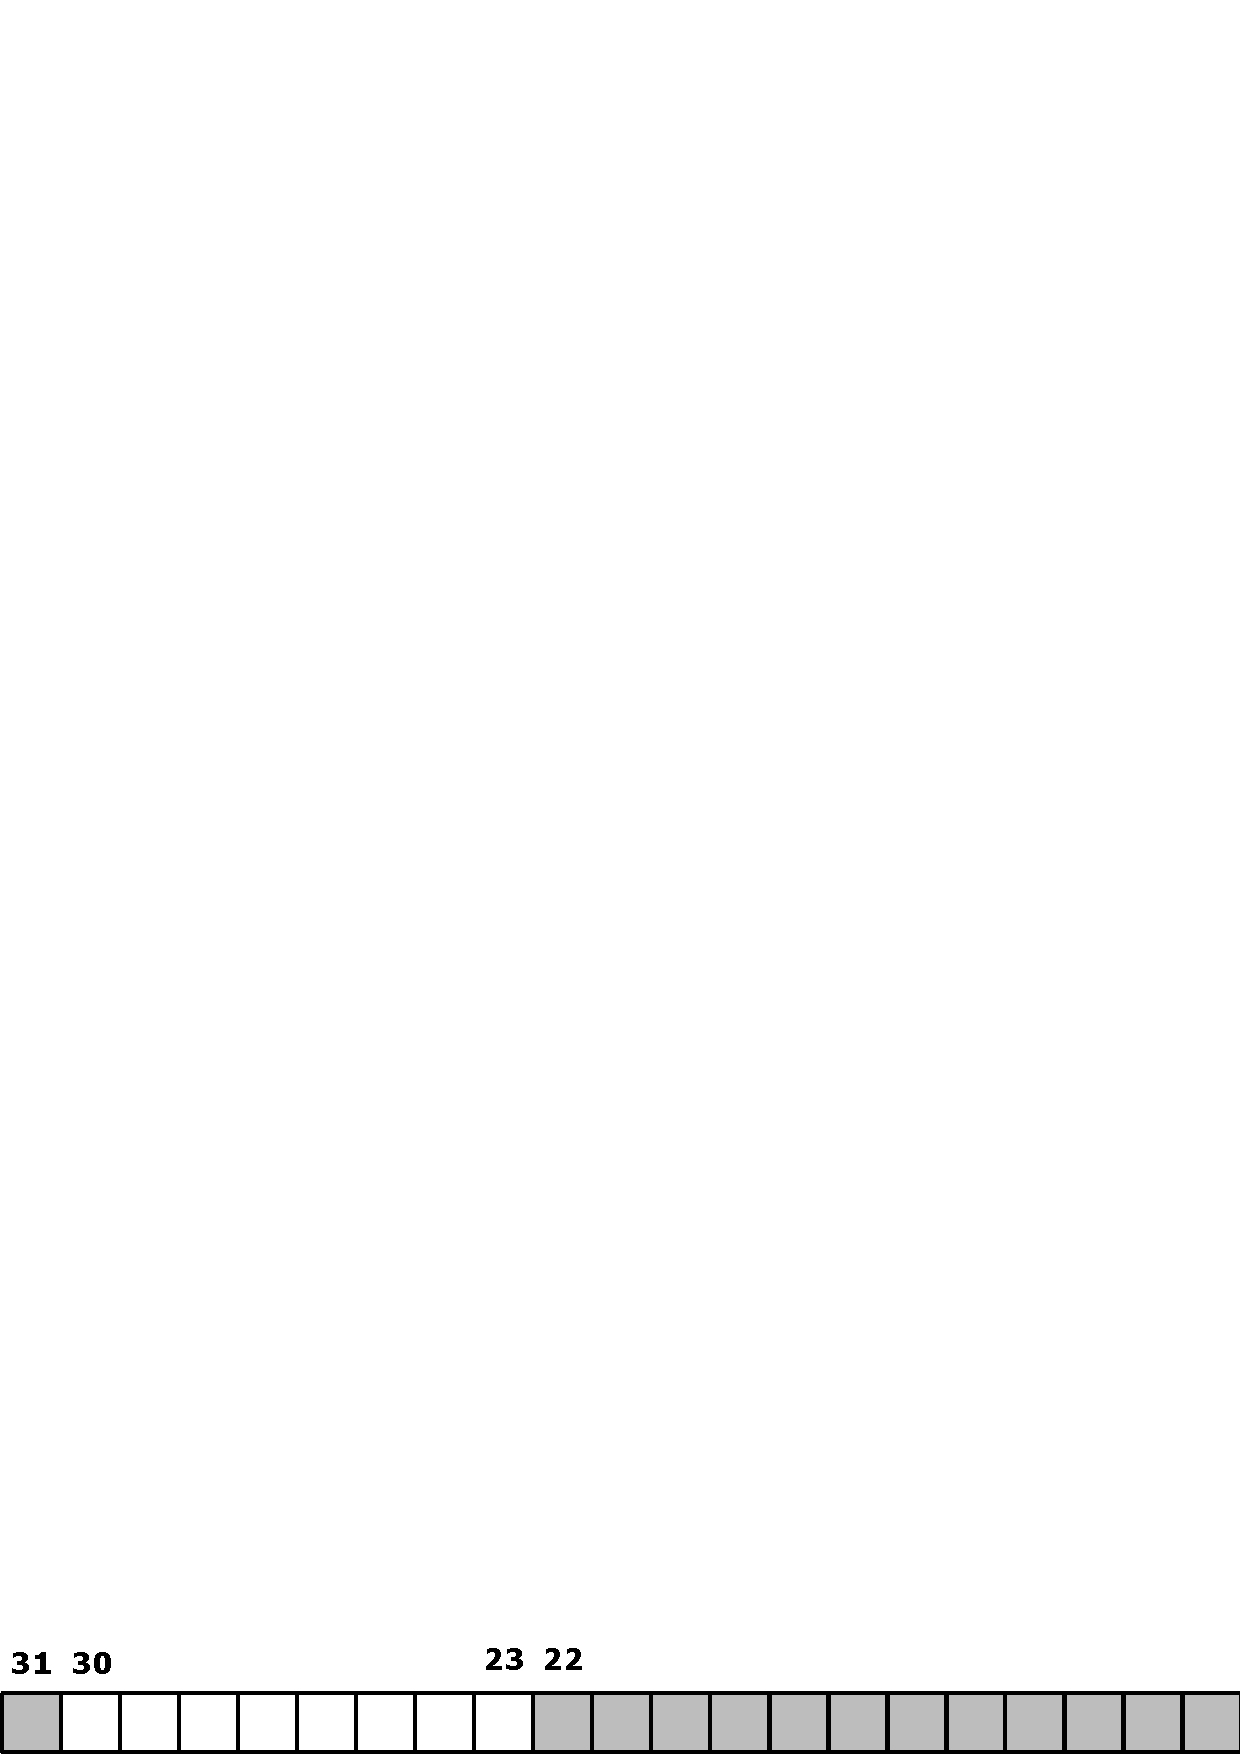
\includegraphics[width=\textwidth]{imgs/drawings/floating_point_layout.pdf}
\caption{Floating Point internals.}
\end{figure}
  \bigskip



\begin{figure}[H]
\centering
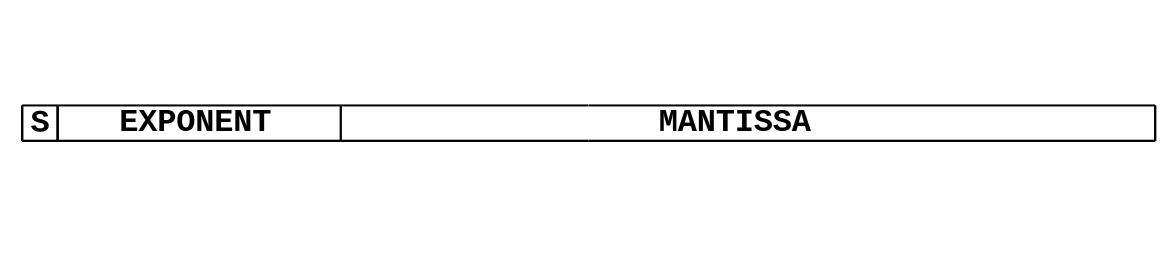
\includegraphics[width=\textwidth]{imgs/drawings/floating_point_math.pdf}
\caption{The three sections of a Floating Point number.}
\end{figure}
  \bigskip  


How numbers are stored and interpreted is usually explained with the formula:\\
\par
\begin{figure}[H]
\begin{equation}\label{eq:fp}
\large
(-1)^S * 1.M * 2^{(E-127)}
\end{equation}
 \caption{How everybody hates floating point to be explained to them.}
\end{figure}
\bigskip  

Although correct, this way of explaining floating point usually leaves programmers completely clueless. I blame this dreadful notation for discouraging legions of programmers, scaring them to the point where they never looked back to understand how floating point actually works. Fortunately, there is a better way to explain it. Instead of Exponent, think of a Window between two consecutive power of two integers. Instead of a Mantissa, think of an Offset within that window.\\ 
\par
  
\begin{figure}[H]
\centering
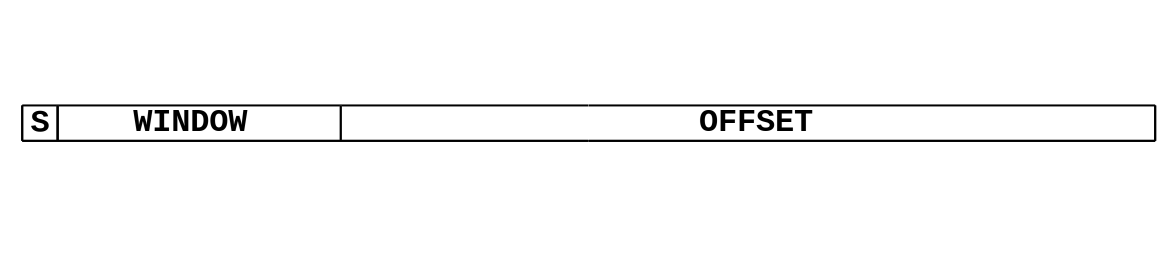
\includegraphics[width=\textwidth]{imgs/drawings/floating_point_intuitive.pdf}
\caption{Alternative Floating Point internals.}
\end{figure}
  \bigskip  
The window tells within which two consecutive power-of-two the number will be: [0,1], [1,2], [2,4], [4,8] and so on (up to [$2^{127}$,$2^{128}$]. The offset divides the window in $ 2^{23} = 8388608 $  buckets. With the window and the offset you can approximate a number. The window is an excellent mechanism to protect from overflowing. Once you have reached the maximum in a window (e.g [2,4]), you can "float" it right and represent the number within the next window (e.g [4,8]). It only costs a little bit of precision.\\


\par \bu{Trivia :} How much precision is lost when the window covers a wider range? Let's take an example with window [0,1] where the 8388608 offsets cover a range of 1 which gives a precision of $(1-0)/8388608=0.00000011920929$. In the window [2048,4096] the 8388608 offsets cover a range of $(4096-2048) = 2048$ which gives a precision $ (4096-2048)/8388608=0.0002$.\\
\par

The next figure illustrates how the number 6.1 would be encoded. The window must start at 4 and span to next power of two, 8. The offset is about half way down the window.

\begin{figure}[H]
\centering
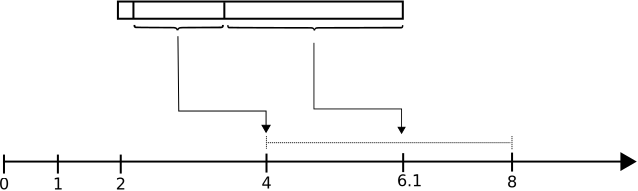
\includegraphics[width=\textwidth]{imgs/drawings/floating_point_window.pdf}

\caption{Value 6.1 approximated with floating point}
\label{fig:fp_internals_window6_1}
\end{figure}
  \bigskip
  
Here is a detailed example to calculates the floating point representation of a number we know well: 3.14.
\begin{itemize}
 \item The number 3.14 is positive  $\rightarrow S=0$.
 \item The number 3.14 is between the power of two 2 and 4 so the floating window must start at $2^1$  $\rightarrow E=128$ (see formula where window is $2^{(E-127)}$).
 \item Finally there are $2^{23}$ offsets available to express where 3.14 falls within the interval [2-4]. It is at $\frac{3.14 -2 }{4 - 2} = 0.57\%$ within the interval which makes the offset $ M = 2^{23}*0.57 = 4781507$
\end{itemize}

Which in binary translates to:

\begin{itemize}
\item S = 0 = 0b
\item E = 128 = 10000000b
\item M = 4781507 = 1001000111101111000011b
\end{itemize}

\begin{figure}[H]
\centering
\includegraphics[width=\textwidth]{imgs/drawings/floating_point_layout_pi.pdf}
\caption{3.14 floating point binary representation.}
\label{fig:fp_internals}
\end{figure}
  \bigskip

The value 3.14 is therefore approximated to 3.14000000000000012.\\

The corresponding value with the ugly formula:

\begin{equation}
3.14 = (-1)^0 * 1.57 * 2^{(128-127)}
\end{equation}

\bigskip

And finally the graphic representation with window and offset:\\

\begin{figure}[H]
\centering
\includegraphics[width=\textwidth]{imgs/drawings/floating_point_window_pi.pdf}

\caption{3.14 window and offset.}
\label{fig:fp_internals}
\end{figure}
  \bigskip

Floating point arithmetic is a powerful tool. It can represent very small or huge values while keeping track of fractional parts of a number, and also protecting from overflow by floating the window when necessary.\\
\par
Floating point is handy, but the drawback is that it is also computationally expensive. The reason is simple. In order to add, subtract, multiply or divide two numbers, they both have to be expressed with the same window. Which means converting one number to the representation used by the other, usually with higher precision than 32 bits (typically 80 bits on Intel FPUs)\footnote{To fully grasp how much processing a FPU does, it helps to read a software implementation. I found Berkeley SoftFloat helpful.}.\\
\par
This is not a problem when everything is hardwired within an hardware floating point unit but it is a big problem for the 386. If you refer back to the architecture diagram you will notice that it only has an ALU. \emph{A 386 doesn't have a hardware Floating Point Unit}. If \cw{float} operations are found in the code, they are emulated in software by the compiler, resulting in terribly slow processing. So slow they are not usable for anything real-time.\\ 
\par


 \textbf{\underline{Trivia :}} Since floating point units were so slow, why did the C language end up with \cw{float} and \cw{double} types ? After all, the machine used to invent the language (PDP-11) did not have a floating point unit! The manufacturer (DEC) had promised to Dennis Ritchie and Ken Thompson the next model would have one\footnote{The Development of the C Language by Dennis M. Ritchie.}. Being astronomy enthusiasts they decided to add those two types to their language.\\
\par


\textbf{\underline{Trivia :}} People who really wanted an hardware floating point unit could buy one. In the 90s the only people who could possibly want one would have been scientists (as per Intel understanding of the market). They were marketed as "Math CoProcessor". Performances were average and price was outrageous\footnote{\$200 in 1993 equivalent to \$350 in 2016.}. As a result, sales were mediocre.\\
\begin{figure}[H]
\centering
  \shadowbox{
      \fullimage{BOX_IntelBOX387SX20.jpg}
  }
\caption{Intel 1991 ad for "Math CoProcessor".}
\label{fig:fp_internals}
\end{figure}



\par
A possible solution to the lack of a hardware floating point unit would have been to multiply an integer by 100 or 1000 to perform fractional operation and then divide to go back to integers. That is unfortunately not possible. On a 386, a multiply (\cw{imul}) instruction takes a minimum of 6-9 cycles and a divide (\cw{div}) is even worse with 22-25 cycles depending if the operands are RAM or register\footnote{Source: http://zsmith.co/intel\_i.html\#imul}.\\ 
\par
As a result, a game engine designer was stuck in an awkward situation with two half solutions to his problem. Integers which were fast but not accurate enough and Floats which were accurate but not fast enough.\\
\par
  






















\section{RAM}
The first CPUs in the Intel x86 family were designed in 1976. A time where RAM was very expensive, the 8080 and 8086 had 16 bit registers with a 20 bit wide address bus capable of addressing 1MiB of RAM. It is difficult to stress how big 1MiB of RAM was in the 70s but as an example, the Apple II and the Commodore 64 both shipped with 64KiB which was enough to write and run amazing things. Sixteen bit registers and 20 bit address bus was plenty even though programming was difficult and required combining two registers to build a pointer. In 1986, the hardware had gotten cheaper and Intel made a departure from the old architecture with its 286 and 386. These new CPUs could be put in what is called "Protected Mode" featuring a 24 bits wide address bus for up to 16 MiB of flat RAM protectable with a MMU\footnote{Memory Management Unit}. The 386 also had 32 bit registers in Protected Mode. To make sure old programs could still run, both processors could be put in "Read Mode" which replicates how the Intel 8080 and 8086 operated: 16 bits registers, 20 bits address bus giving 1MiB addressable RAM with segmented addressing.\\
\par
For compatibility reasons all PCs must start in Real Mode. You may assume that programmers of the 90s promptly switched the CPU to Protected Mode to unleash the full potential of the machines and ditch the 20-year-old Real Mode. Unfortunately, there was a major obstacle: the operating system MS-DOS by Microsoft Corporation.
  






  \subsection{DOS limitations}
  Microsoft Corporation highly valued the applications running on their operating systems. As a business priority, they were adamant to never break anything with a new system\footnote{"Tales of Application Compatibility", Old New Thing by Raymond Chen}.  Since many applications were written during the 80s on machines having only Real-Mode, DOS 5.0 kept running that way and as a result its routines and system calls were incompatible with Protected Mode. This created an awkward situation where the \emph{de-facto} operating system delivered with every machine sold prevented programmers from using the machine at its full potential. Developers were forced to ignore all the features of their 1992 CPU and use it like a very fast Intel 8086 CPU from 1976. They were thus limited to the following characteristics: \\
\begin{itemize}
\item ALU
\item 15 registers:
\begin{itemize}
  \item 16-bit General Purpose Registers: AX, BX, CX, DX
  \item 16-bit Index Registers: SI, DI, BP, SP
  \item 16-bit Program Counter: IP
  \item 16-bit Segment Registers: CS, DS, ES, FS, GS, SS
  \item 16-bit Status Register
\end{itemize}
\item Up to 1MiB of RAM
\end{itemize}


\bigskip

 \textbf{\underline{Trivia :}} One year earlier, in 1991, a student from the University of Helsinki started working on a hobby ("nothing big") of his. An operating system which contrary to DOS was able to use the CPU in Protected Mode and take advantage of the MMU and the 32 bits registers. It would become Microsoft's worse nightmare. Linus Torvalds had just started what would become Linux.



  \subsection{The infamous Real Mode: 1MiB RAM limit}
  With Protected Mode unavailable, developers of 1991 programmed like it was 1976. With a 20 bits wide address bus offering only 1MiB of addressable RAM. No matter how much memory was installed on the machine, only 1MiB could be addressed. To top it all off, addressing had to be done not with the 32 bits registers available but by combining two 16 bits registers together. One was the segment, the other an offset within that segment. Hence the name: '16 bits segmented programming'.

  \bigskip
The memory layout is as follow:\\
\begin{itemize}
\item From 00000h to 003FFh : the Interrupt Vector Table.
\item From 00400h to 004FFh : BIOS data.
\item From 00500h to 005FFh : command.com+io.sys.
\item From 00600h to 9FFFFh : Usable by a program (about 620KiB in the best case). 
\item From A0000h to FFFFFh : UMA (Upper Memory Area): Reserved to bios ROM, video card and sound card mapped I/O.
\end{itemize}

\begin{figure}[H]
\centering
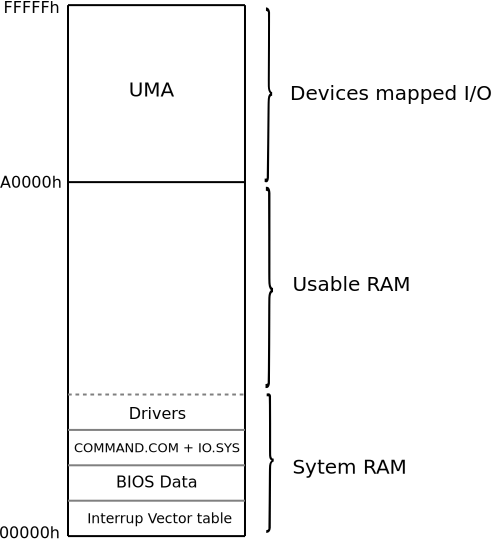
\includegraphics[width=\textwidth]{imgs/drawings/real_mode.pdf}

\caption{First 1MiB of RAM layout.}
\label{fig:fp_internals}
\end{figure}


Out of the original 1024KB, only 640KiB (called Conventional Memory) were usable to a program. 384KiB were reserved for the UMA and every single driver installed (\codeword{.SYS} and \codeword{.COM})  took away from the remaining 640KB.

\bigskip

\textbf{\underline{Trivia :}}  In France people had to load KEYBFR.SYS driver so their AZERTY keyboard keys would be properly mapped. The driver consumed a whopping 5KiB of Conventional Memory. Needless to say French people learned pretty quickly that god mode was IDDAD\footnote{Invincibility mode in Doom is IDDQD on a qwerty keyboard but IDDAD on an azerty keyboard without the French driver loaded.}.\\
\par





\subsection{The infamous Real Mode: 16 bit Segmented addressing}
With a 20 bits address bus and registers too small to contain a whole address (they are 16 bits wide), Intel had to come up with an addressing system. Their solution was to combine two 16 bits registers, one designating a segment and the other an offset within that segment.\\
\par
\begin{figure}[H]
\centering
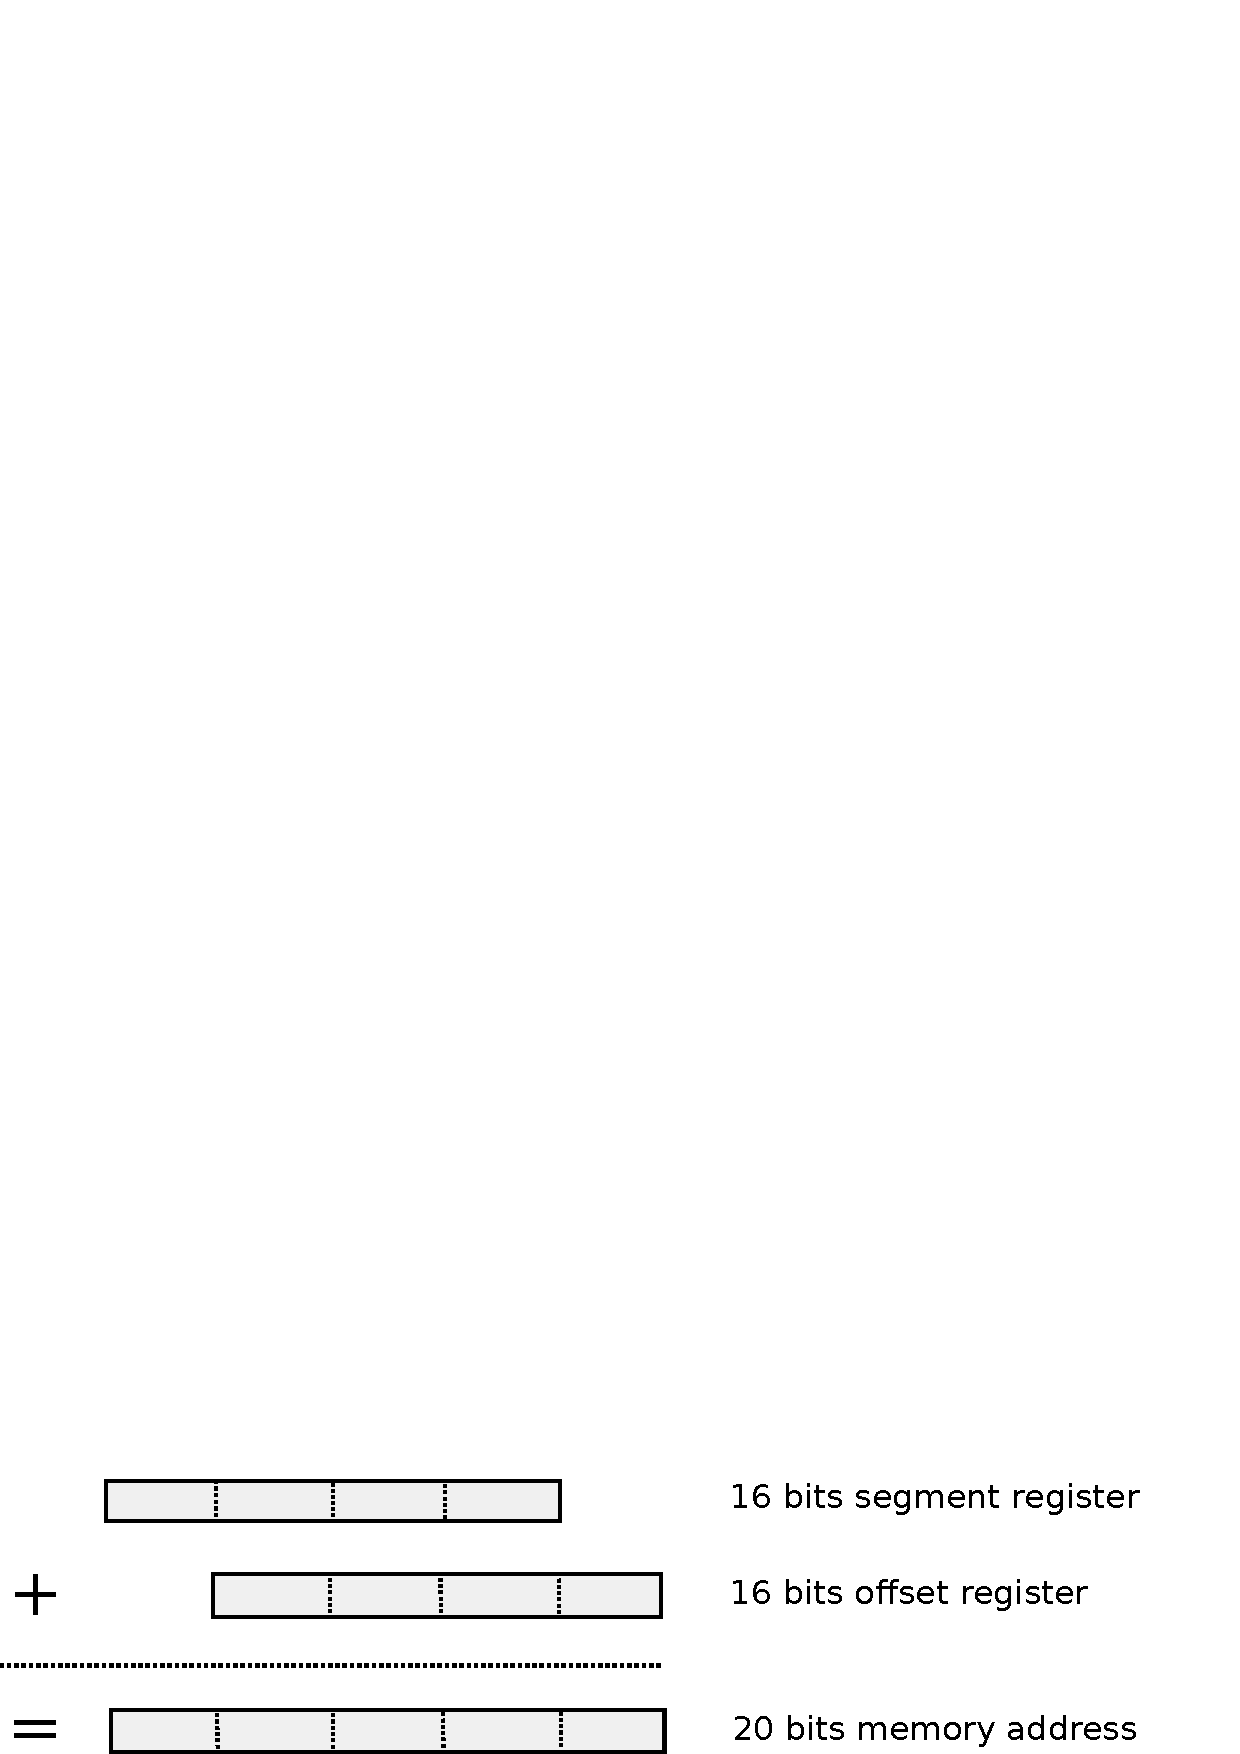
\includegraphics[width=\textwidth]{imgs/drawings/register_combination_20_bits_address.pdf}
\caption{How registers are combined to address memory.}
\label{fig:register_comb_to_20_bits}
\end{figure}
\par
There are two kinds of pointers: \cw{near} and \cw{far}. A \cw{near} pointer is 16 bit and considered \emph{fast} because it can be used as is (but it only allows a \cw{jmp} in the current code segment). A \cw{far} pointer can access anything and allows a \cw{jmp} anywhere but it is slower since a 16 bit segment register has to be shifted left 4 bits and combined with the other 16 bit offset register to form a 20 bits address.\\

That may not sound too bad, but in practice this segmented addressing leads to many issues.
The least problematic is about the language. Since C was invented on a flat memory machine, it had to be augmented by PCs compiler manufacturers. That is how the \codeword{near} and \codeword{far} keywords came to existence. To build pointers, a set of macro are provided, respectively \codeword{FP\_SEG} and \codeword{FP\_OFF}. Of course \cw{libc} is also "different": \cw{malloc} returns a \cw{near} pointer and therefore can only allocate up to 64kB. To get more than 64K, \cw{farmalloc} is needed.\\
\par
The larger issue is that two pointers referring to the same address can fail an equality test. In this model, the 1MiB of RAM is divided in 65536 paragraphs by the segment pointer. A paragraph is 16 bytes but an offset can be up to 65536 which results in many overlaps. It is easy to understand with the following examples.\\
\par
Pointer A defined as:\\
\par
\begin{minipage}{\textwidth}
\lstinputlisting[language=C]{code/pointer_madness1}
\end{minipage}

\bigskip

Pointer B defined as:\\
\par
\begin{minipage}{\textwidth}
\lstinputlisting[language=C]{code/pointer_madness2}
\end{minipage}

\bigskip

Pointer C defined as:\\
\par
\begin{minipage}{\textwidth}
\lstinputlisting[language=C]{code/pointer_madness3}
\end{minipage}

As defined, A, B and C all point to the same memory location however they will fail a comparison test.\\

\begin{minipage}{\textwidth}
\lstinputlisting[language=C]{code/pointer_madness.c}
\end{minipage}
\par
Will output:\\

\begin{minipage}{\textwidth}
\lstinputlisting{code/pointer_madness_output.txt}
\end{minipage}
\par

With this system, pointer arithmetic must also receive careful consideration. A \cw{far} pointer increment only increments the offset, not the segment. If you iterate on an array larger than 64KiB you will end up wrapping around. You could use yet an other type of pointer \cw{int huge*} to make pointer arithmetic work beyond 64k but really, nobody wants to go there.




  \subsection{Extended Memory}

The 20 bit address bus of Real Mode limits the addressable RAM to 1MB. Machines of 1992 came equipped with more, typically 2MiB and even sometimes 4MiB for the most fortunate customers. This memory located beyond the addressable space is called "Extended Memory". The workaround at the time to access these resources was to install specialized drivers\footnote{See CONFIG.SYS in the appendice.}.\\
\par
Unfortunately extended memory access was not standardized. Users could load either of the drivers provided with DOS:
\begin{itemize}
\item Expanded Memory Specification (EMS) drivers: EMM368.SYS.
\item eXtended Memory Specification (XMS) drivers: HIMEM.SYS.
\end{itemize}

Or they could have no idea they had to install a driver, load nothing at startup, and not use any of the RAM beyond 1MB. This use case was a big issue. Many customers could not understand why, even though they had installed (extremely expensive\footnote{In 1992, 4MiB of RAM cost \$149 which adjusted to inflation would be \$256 in 2016.}) megabytes of RAM on their machine, the game they just purchased would refuse to start up claiming "Not enough memory". id Software had to publish an explanation (see Appendix "\nameref{chap:barrier640}") along with the game to make it clear it was not their fault.\\
\par
How are these drivers working? After all, how does one access RAM outside of the addressable space? On the 386 the driver switched the CPU into protected mode, performed whatever was asked and switched the CPU back to real mode. On the 286, there was no way to switch back the CPU to real mode\footnote{The first hack to do the impossible put a magical value into a special memory location to prevent the BIOS from reinitializing the computer after a reset, and then caused a reset through the i8042 keyboard controller which would externally reset the CPU. Other techniques involved generating a triple fault (faulting in a fault handler, usually by invalidating the IDTR and causing an interrupt). Using the triple fault was much faster. Going through the keyboard controller took almost a millisecond but the triple fault performed in a hundred microseconds} but there was an undocumented \cw{LOADALL} instruction which allows to manipulate an hidden register offsetting all RAM access.
\footnote{"HIMEM.SYS, unreal mode, and LOADALL": http://www.os2museum.com/wp/himem-sys-unreal-mode-and-loadall/}

\begin{figure}[H]
\centering
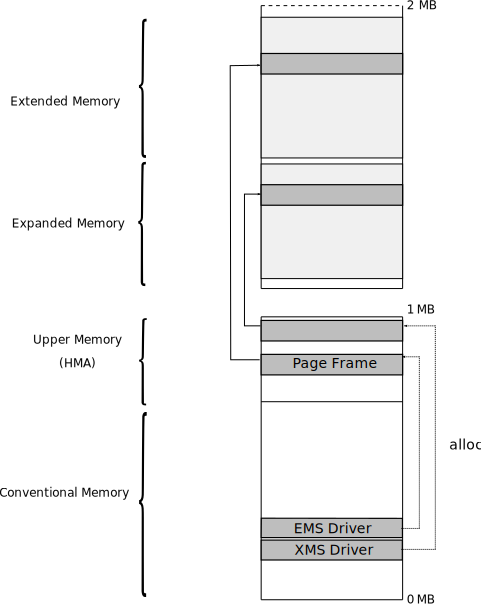
\includegraphics[width=\textwidth]{imgs/drawings/expanded_ram.pdf}
\caption{Expanded/Extended memory layout}
\label{fig:ems_xms_layout}
\end{figure}


\textbf{\underline{Trivia :}}  As of 2016, more than thirty five years after the introduction of the 8086, in the name of backward compatibility, all PCs in the world still start in Real Mode. A bootloader switches them to Protected Mode, loads the kernel, and then real startup can begin.


\subsubsection{EMS API}

The EMS driver opens a window beyond the addressable RAM, as shown in Figure \ref{fig:ems_xms_layout}. The idea revolves around memory mapping. The driver allow for manipulating four units of 16KiB called "pages" via a 64KiB area called "Page Frame". Upon request to the driver, a frame can be swapped into the page frame.\\
\par



\subsubsection{XMS API}
The XMS driver works like \cw{malloc}, it provides operations such as allocate, free, realloc and the most important one move which allows to copy from extended RAM to conventional RAM\footnote{eXtended Memory Specification (XMS) July 19, 1988.}.








\subsubsection{A system "Impossible to love"}
At this point, if you are puzzled by the CPU and its design you are not alone. Over the years I came across many ways to describe this madness but three particularly stand out.\\
\par
 \begin{fancyquotes}
   The x86 is an architecture that is difficult to explain and impossible to love.\\
   \par
\textbf{David Patterson \& John Hennessy - Computer Organization and Design.}
 \end{fancyquotes}\\
\par
And:\\
\par
 \begin{fancyquotes}
    That sounds odd, but Intel built it, Microsoft wrote it, and DOS grew up around it.\\
   \par
\textbf{Eccles-Jordan Trigger - Codeproject.com.}
 \end{fancyquotes}\\
\par
 \begin{fancyquotes}
    Software poison.\\
   \par
\textbf{Steve Morris - Co-Architect of the Intel 8086.}
 \end{fancyquotes}\\


\par
\bu{Trivia :} 640KiB was all a game could have for executable code. But people writing compilers got clever. Strike Commander (a famous flight arcade game released in 1993) executable is 745kB, which obviously doesn't fit in Conventional Memory. The trick was to use a technique of "overlays". The compiler inserted instructions at compile time to detect when the CPU IP\footnote{Instruction Pointer} was about to move beyond a page. These instructions swapped code segment from RAM to HDD and issued a \cw{jmp} to reset the CPU at the beginning of the next page.

















\section{Video}

PCs were connected to CRT monitors. Big, heavy, small diagonal, cathodic ray based with curved surface screens. Most monitors had a 13" diagonal with a 4:3 aspect ratio. To give you an idea of the size, Figure \ref{fig:int_layout} shows a comparison between a 13" CRT from 1992 and a 23" LCD display from 2014.\\

\begin{figure}[H]
\centering
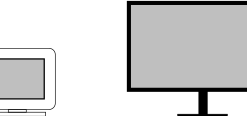
\includegraphics[width=\textwidth]{imgs/drawings/crt_lcd.pdf}
\caption{CRT (left) vs LCD (right)}
\label{fig:lcd_vs_crt}
\end{figure}

\begin{minipage}{.4\textwidth}
\textbf{\underline{Trivia :}} How big and heavy could a CRT be? The InterView 28hd96 by Integraph weighed 45kg (99.5lb). For comparison, a modern DELL LCD 27" weights 7.8kg (17lb).\\
\par
In the photo on the right : John Carmack in 1996 working on an InterView 28hd96 while programming Quake 2 using Visual Studio C++.\\
\end{minipage}
\begin{minipage}{.6\textwidth}
\begin{figure}[H]
  \begin{flushright}
       %\frame{
       \scaledimage{0.9}{johnCarmackWorking.png}
       %}
    \end{flushright}
\end{figure}
\end{minipage}

\par
The main issue in this system is that CRTs are analogic systems while computers are digital. An interface is needed between the two and it came as a series of chipsets called "Adapters". 

  \subsection{History of Video Adapters}

The first adapter of the family was released in 1981. The Monochrome Display
   Adapter (\codeword{MDA}) offered two colors allowing text with 80 columns by 25 lines.  Not great, but it had the merit to be standard on every PC. Many other systems followed over the years, each of them preserving backward compatibility.
\bigskip
  
 \begin{figure}[H]
\centering  
\begin{tabularx}{\textwidth}{ X  Y }
  \toprule
  \textbf{Name} &  \textbf{Year Released} \\
  \toprule \codeword{MDA}
   (\textbf{M}onochrome
   \textbf{D}isplay
   \textbf{A}dapater) & 1981 
   \\ \codeword{CGA}
   (\textbf{C}olor
   \textbf{G}raphics
   \textbf{A}dapter) & 1981 
    \\ \codeword{EGA}
   (\textbf{E}nhanced
   \textbf{G}raphics
   \textbf{A}dapter) & 1985
   \\ \codeword{VGA}
   (\textbf{V}ideo
   \textbf{G}raphics
   \textbf{A}rray)  & 1987
    \\
  \toprule
\end{tabularx}
\caption{Video interface history.}\label{fig:vga_history}
\end{figure}

Each iteration added new features and by 1991 the ubiquitous graphic system was VGA. All video cards installed on PCs had to follow the standard set by IBM. The universality of that system was a double-edged sword. On one side developers had to program for only one graphic system. But on the other side, there was no escaping its shortcomings.\\

\begin{figure}[H] 
  \centering 
  \fullimage{hardware/suntra_trident_tvga8800br.png} 
  \caption{A VGA card Trident 8800 (8 bits ISA). Courtesy of \cw{vgamuseum.info}.}
\end{figure}
\par
\begin{figure}[H] 
  \centering 
  \fullimage{hardware/diamond_stealth_vram_revb2.png} 
  \caption{A VGA card Diamond Stealth (16 bits ISA). Courtesy of \cw{vgamuseum.info}.}
\end{figure}
\bu{Trivia :} There was no GPU market back then. Since all video cards "only" had to be VGA compatible with 256KiB of RAM, most people just bought the cheapest thing available. Note however that some cards had an 8 bits ISA bus connector (like the Trident) and some had an ISA 16 bits connector like the Diamond, making the Diamond transfer data twice as fast.\\
\par




\subsection{VGA Architecture}

VGA can be summarized as three major systems with input, storage, and output systems:\\

\begin{itemize}
\item The Graphic Controller and Sequence Controller controlling how the VGA RAM is accessed (the CPU-VRAM interface)
\item The framebuffer (the VRAM) made of not one memory bank of 256KiB but four memory banks of 64KB
\item The CRTC Controller and the DAC\footnote{Digital To Analog Converter} taking care of converting the Palette indexed framebuffer to RGB and then to analogical signal (interface VRAM-CRT)
\end{itemize}

The most surprising part of the architecture is obviously the framebuffer. Why have four small fragmented banks instead of one big linear one?\\
\par
The first part of the explanation comes from backward compatibility. The version before VGA, EGA, had only 64KiB of RAM. It was very easy to design a backward compatible system that used only one bank of 64KB.\\
\par
But the real reason was RAM latency and the need for a minimum bandwidth. A CRT running at 70Hz and displaying 640x480 in 16 colors needs a pixel every 1/(640*480*70)th of a second. At this resolution, one pixel is encoded on 4 bits. Each nibble is translated to a 666 RGB color by the DAC. That encoding divides bandwidth by six, but you still need one byte every 91 nano-seconds. Unfortunately, RAM access latency was 200ns. Not nearly fast enough\footnote{Computer Graphic: Principles and Practice 2nd Edition, page 168} to refresh the screen at 70hz, so the DAC would starve. If latency could not be reduced, the throughput could still be improved by reading from four banks at the time. Reading in parallel give an amortized RAM latency of 200/4 = 50ns which is fast enough.\\
\par
Keep in mind that this architecture reduced the penalty of read operations, but plotting a pixel in the framebuffer with a write operation was still slow. To write to the VRAM as little as possible was very important in order to maintain a decent framerate. 


\begin{figure}[H]
\centering
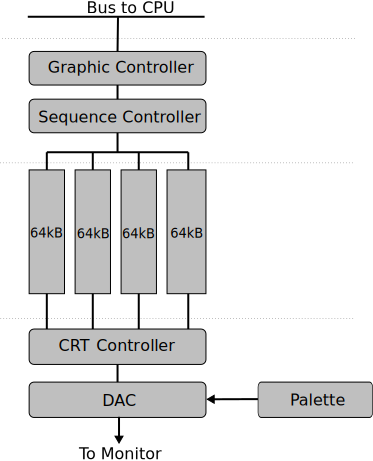
\includegraphics[width=\textwidth]{imgs/drawings/vga.pdf}
\caption{Video Graphic Array Architecture.}
\label{fig:vga_arch}
\end{figure}




\subsection{VGA Planar madness}

Four memory banks grant enough throughput to reach high resolutions at 70Hz. The price is complexity of programming, as acknowledged by even the best programmers of the time.\\

 \begin{fancyquotes}
   Right off the bat, I'd like to make one thing perfectly clear: The VGA is hard-sometimes very hard-to program for good performance.
 \bigskip \\
\textbf{Michael Abrash - Graphic Programming Black Book}
 \end{fancyquotes}
 \\
\par
The first problem with this design is that it is unintuitive. There is no linear framebuffer and figuring out which byte corresponded to what pixel on screen is difficult.\\
\par
 This type of architecture is called "planar" and to write four pixels next to each other on a line on the screen, you have to write one byte in each bank. Each of these banks are mapped at the same UMA memory address. The layout is better explained with a drawing.\\
\par
\begin{figure}[H]
\centering
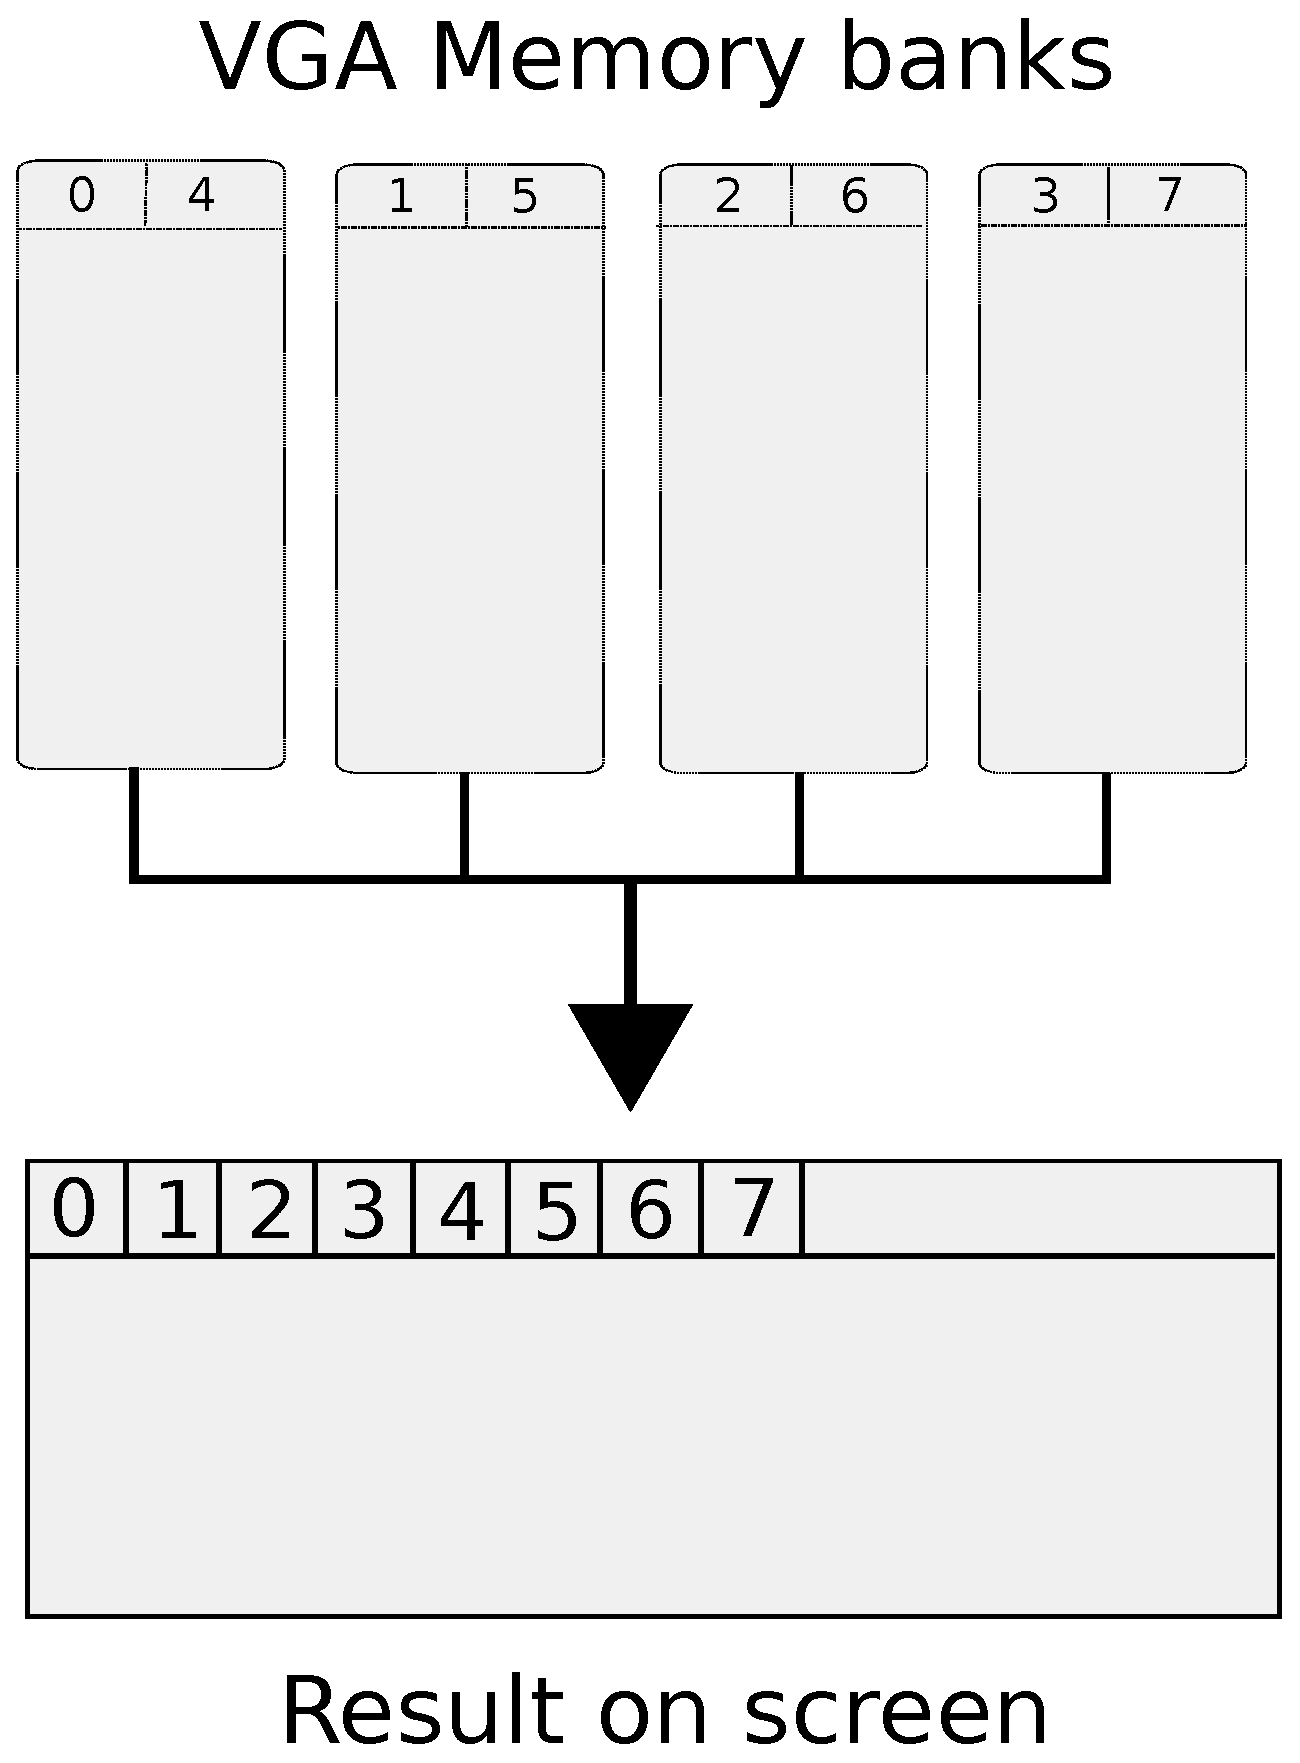
\includegraphics[width=.6\textwidth]{imgs/drawings/vga_ram_screen_layout.eps}
\label{fig:vga_arch}
\end{figure}

 

\par
In order to configure this mess of planes and the controllers, 300 poorly documented internal registers must be set. Needless to say few programmers dove into the internals of the VGA. The first figure describing its architecture was actually deceptively simplified. The IBM VGA reference documentation had its own drawing but it only illustrated the difficulty of the system.\\
 \begin{figure}[H]
\centering
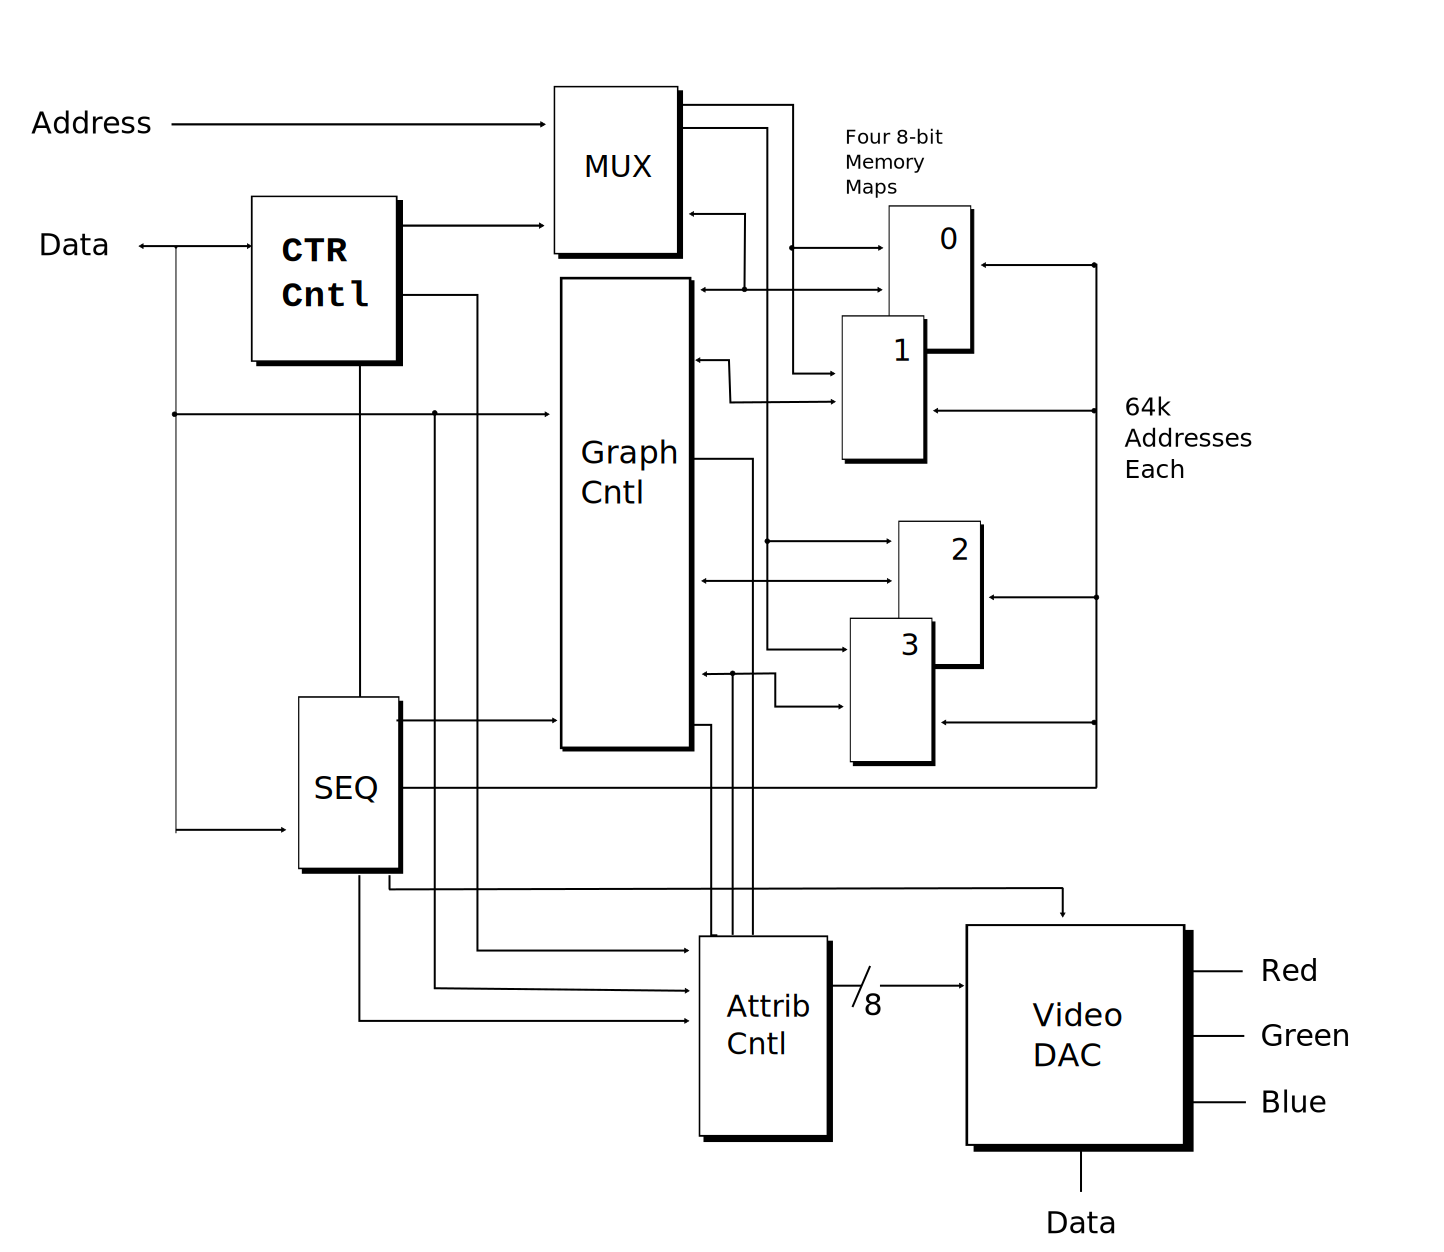
\includegraphics[width=\textwidth]{imgs/drawings/ibm_vga.pdf}
\caption{IBM's VGA Documentation}
\label{fig:ibm_vga}
\end{figure}

\bigskip



To compensate for the complexity, IBM provided a routine to initialize all the registers via one simple BIOS call. A configuration can be selected out of 15 available (a configuration is called a "mode") with an associated resolution, number of colors, and memory layout.

\subsection{VGA Modes}

The BIOS can be called to configure the VGA as follows.

\begin{figure}[H]
\centering
\begin{table}[H]
\begin{tabularx}{\textwidth}[c]{llllr}
\hline
\textbf{Mode} & \textbf{Type} & \textbf{Format} & \textbf{Colors}          & \multicolumn{1}{l}{\textbf{RAM Mapping}} \\ \hline
0             & text          & 40x25           & 16 (monochrome) & b8000h                                \\ \hline
1             & text          & 40x25           & 16                       & b8000h                                \\ \hline
2             & text          & 80x25           & 16 (monochrome) & b8000h                                \\ \hline
3             & text          & 80x25           & 16                       & b8000h                                \\ \hline
4             & CGA Graphics  & 320x200         & 4                        & b8000h                                \\ \hline
5             & CGA Graphics  & 320x200         & 4 (monochrome)  & b8000h                                \\ \hline
6             & CGA Graphics  & 640x200         & 2                        & b8000h                                \\ \hline
7             & MDA text      & 9x14            & 3 (monochrome)  & b0000h                                \\ \hline
0Dh           & EGA graphic   & 320x200         & 16                       & A0000h                                \\ \hline
0Eh           & EGA graphic   & 640x200         & 16                       & A0000h                                \\ \hline
0Fh           & EGA graphic   & 640x350         & 3                        & A0000h                                \\ \hline
10h           & EGA graphic   & 640x350         & 16                       & A0000h                                \\ \hline
11h           & VGA graphic   & 640x480         & 2                        & A0000h                                \\ \hline
12h           & VGA graphic   & 640x480         & 16                       & A0000h                                \\ \hline
13h           & VGA graphic   & 320x200         & 256                      & A0000h                                \\ \hline
\end{tabularx}
\end{table}
\caption{VGA Modes available.}\label{fig:vga_modes}
 \end{figure}
 
 Programmers referenced VGA modes by their ID. It was a common thing to see tutorials about Mode 12h or Mode 13h, which were the two most appealing modes for game programming.


 \subsection{VGA Programming: Memory mapping}
To write to the VRAM the 1MiB address space maps 64KiB starting as indicated in the Mode table. In mode 13h for example, the VRAM is mapped from 0xA0000 to 0xAFFFF. The first question that may pop in your mind is "How to access 256KiB of RAM with only 64KiB of address space?". The answer is: "bank switching". Write and Read operations are routed based on a mask register indicating which bank should be read or written.\\
\par
 \begin{figure}[H]
\centering
  
      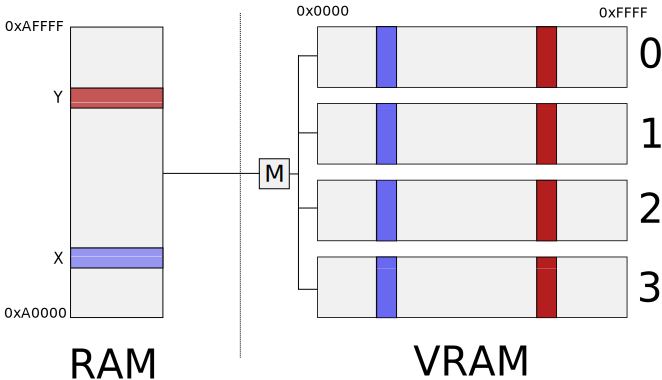
\includegraphics[width=\textwidth]{imgs/drawings/ram_to_vga_mapping.pdf}
    
\caption{Mapping PC RAM to VGA VRAM banks.}
\end{figure}



 

 \subsection{VGA Programming: Mode 12h}
 The first mode commonly considered for game programming is Mode 12h. It offers a resolution of 640x480 at 70hz with 16 colors from a palette. Each pixel is encoded in 4 bits (a nibble) spread across the four banks. To write the color of the first pixel, a developer has to write the first bit of the nibble in plane 0, the second in plane 1, the third in plane 2 and the fourth in plane 3. The CRT Controller then reads 4 bytes at a time (one from each plane) resulting in 8 pixels on screen.\\
\par
\begin{figure}[H]
\centering
 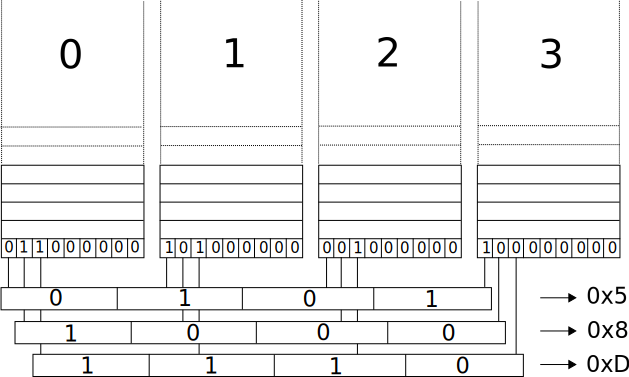
\includegraphics[width=\textwidth]{imgs/drawings/mode12h.pdf}
\caption{VGA banks layout in mode 12h.}
\end{figure}
\par

The only good thing about this mode is that it has square pixels. The 640x480 aspect ratio matches the 4:3 of a CRT so there is no distortion of the framebuffer when it is output to the screen. But pretty much everything else is bad:\\
\begin{itemize}
\item No double buffer: 640X480/2 = 0x25800 bytes which is more than half the 256KiB (0x40000) of VRAM available.
\item The high resolution is actually a drawback for a 3D engine since more pixels means more calculations and more drawing.
\item 16 colors looks really, REALLY ugly.
\end{itemize}

 \begin{figure}[H]
\centering
 \fullimage{wolf3d_ega.png}
 \caption{Wolfenstein3D in 16 colors}
\end{figure}





 
  \subsection{VGA Programming: Mode 13h}
  Mode 13h is far more appealing since it offers a lower resolution of 320x200 with 256 colors at 70Hz. It also has the advantage of faking linear buffer. A special chip called Chain-4 uses the lower 2 bit of the RAM address to automatically program the mask and route the operation to the appropriate VRAM bank. This convenience mechanism was originally added because Mode 13h was meant to display static images and a linear address space made it easy for developers to copy from RAM to VRAM.\\
  \par
 \begin{figure}[H]
\centering
      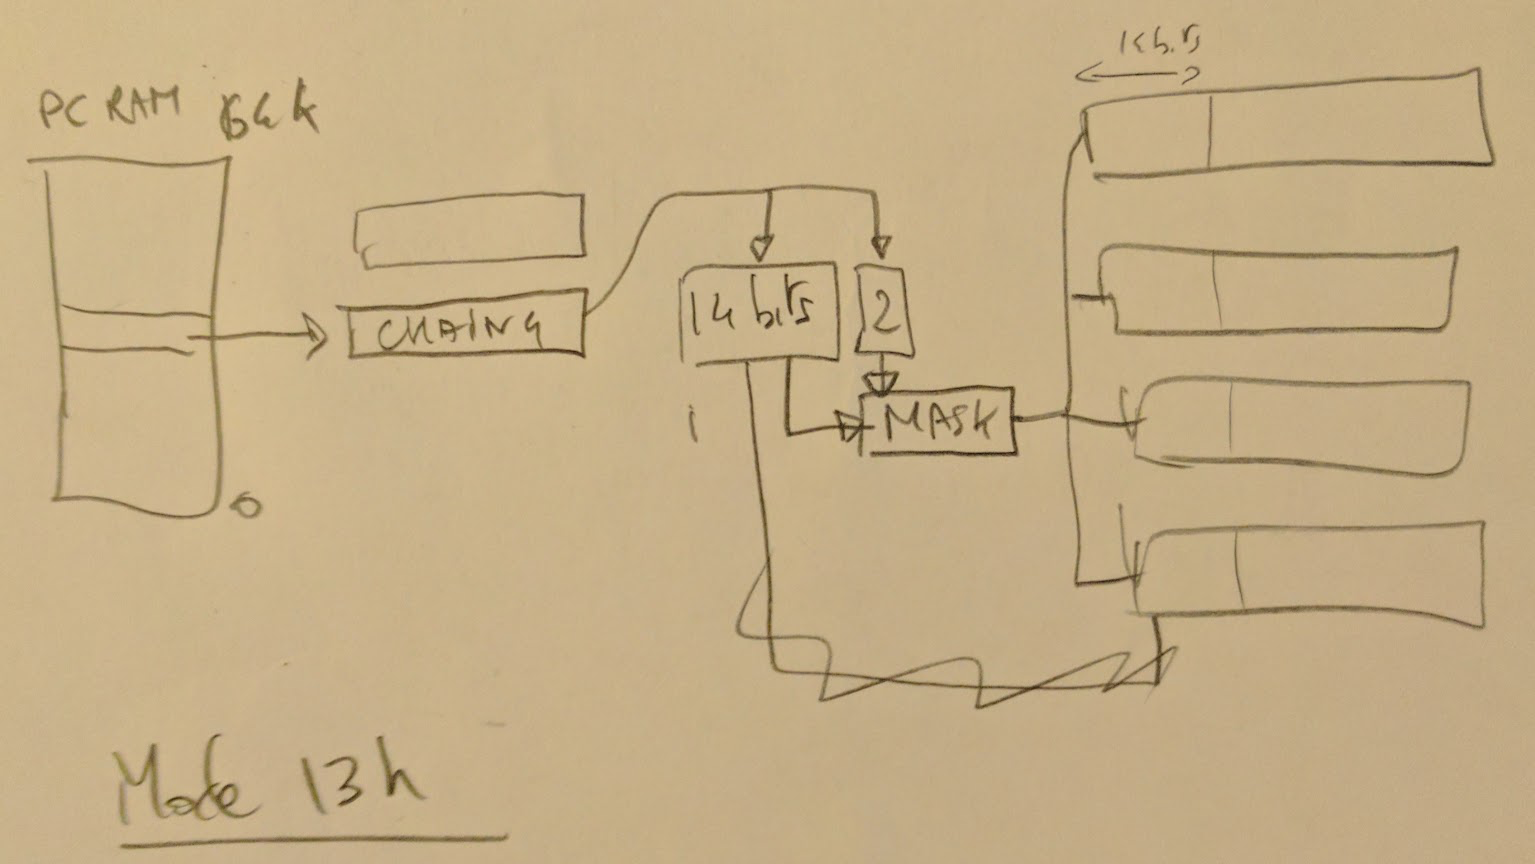
\includegraphics[width=\textwidth]{imgs/drawings/mode_13h.pdf}
\end{figure}
\par

When writing or reading a value V at address K in RAM, the Chain-4 breaks the address down into two parts:
\begin{itemize}
\item The 2 low bits are used to configure the mask automatically. Hence 0x00 goes to bank 0, 0x01 to bank 1, 0x10 to bank 2 and 0x11 to bank 3.
\item The 14 high bits are right shifted by two bits and used as offset in the bank.
\end{itemize}
  \par
  For example, writing at 0xABF13 in RAM would result in writing in bank 3 at offset 0xBF13 >> 2 = 2FC4. Since this is all hardwired in the Chain-4, this extra work is fast and totally invisible to the user.
 \begin{figure}[H]
\centering
      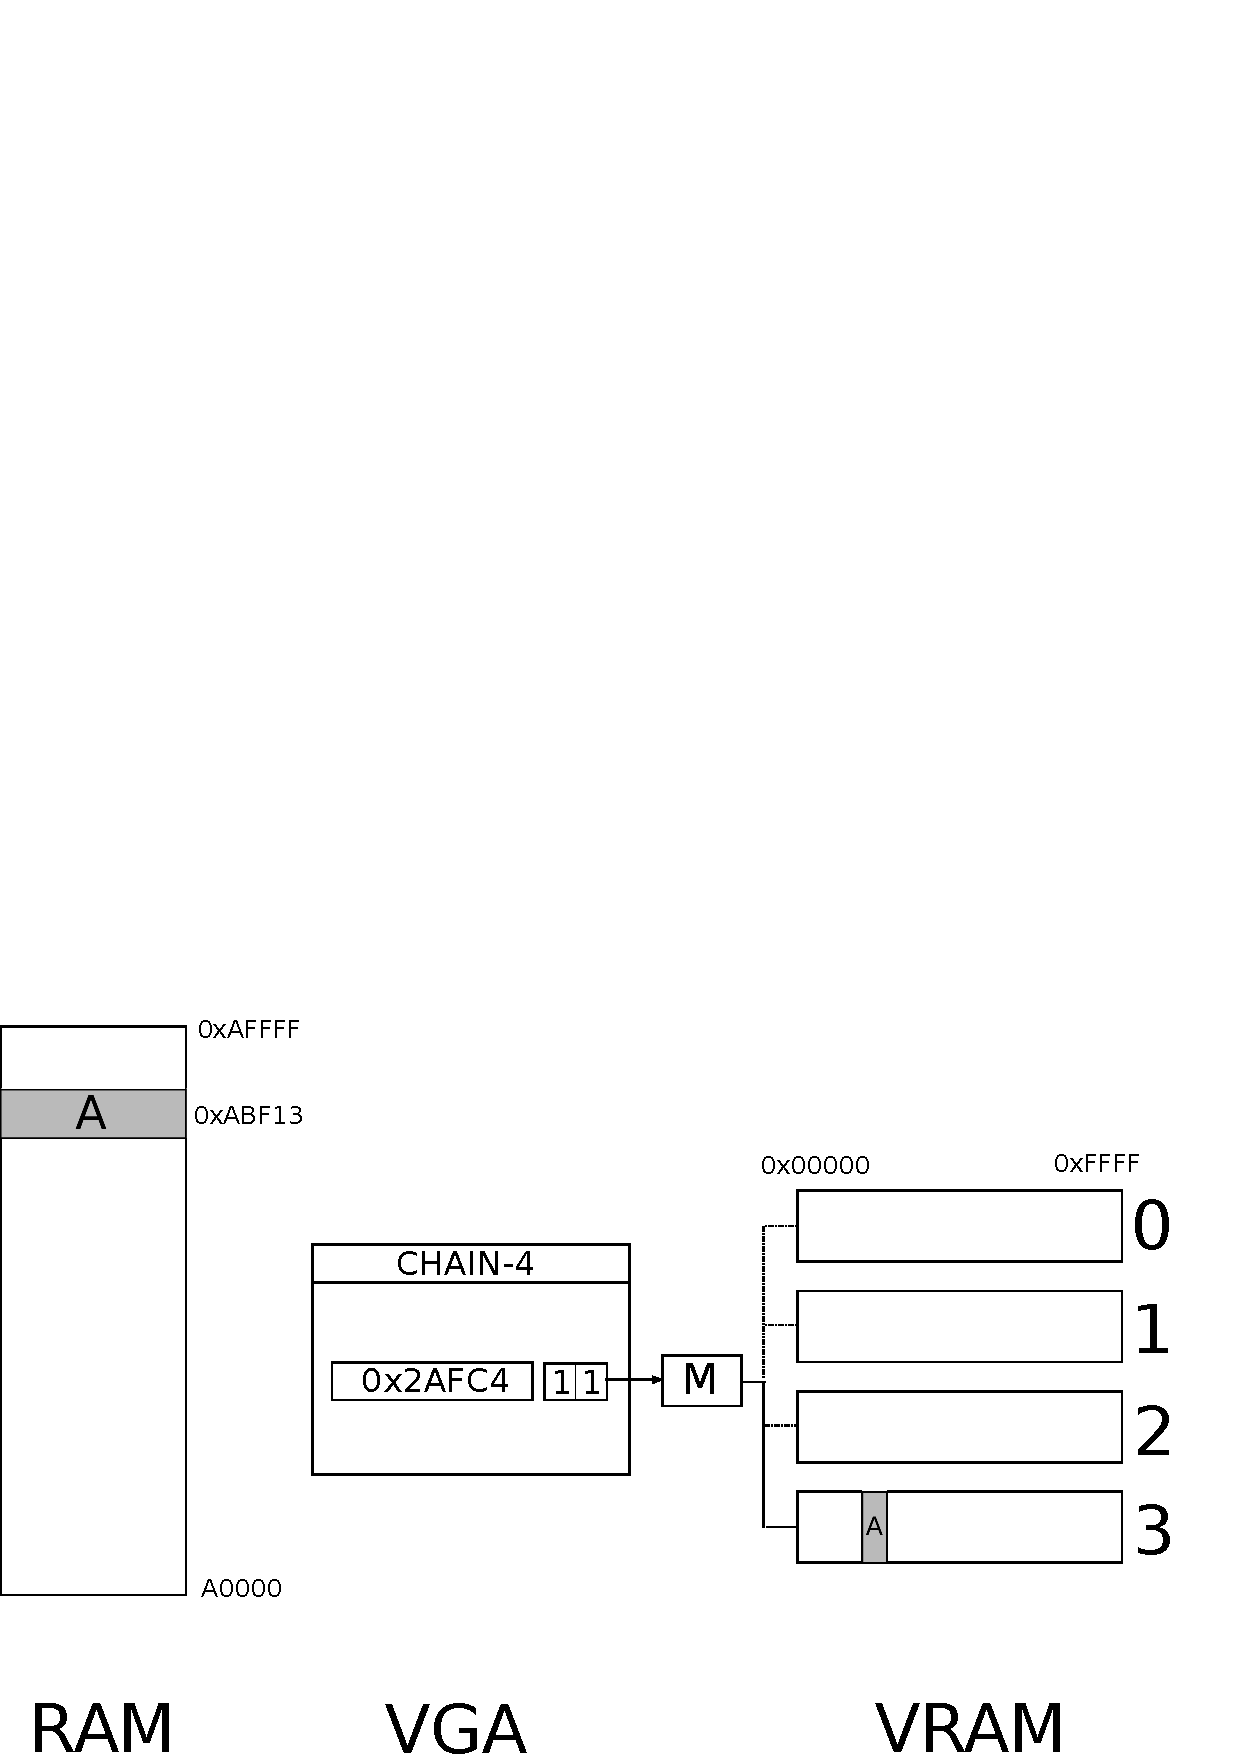
\includegraphics[width=\textwidth]{imgs/drawings/mode_13h_example.pdf}
\end{figure}
\par
The side effect of this convenience mechanism is that 75\% of the RAM is wasted (since only 14 bits are usable for offset).\\

   \subsubsection{Setup}
  To setup the VGA in Mode 13h using the BIOS is incredibly easy:\\
  \par
  \lstinputlisting[ language={[x86masm]Assembler}]{code/vga_mode13.asm}
  
  \par
  The \codeword{int 10} instruction is a software interrupt caught by the BIOS routine in charge of graphic setup. It looks up the \codeword{ax} register to setup all 300 VGA register with the corresponding mode. After the VGA is initialized one can write to the mapped memory at \cw{0xA0000}. It is simpler to follow with a code sample; here is some code to clear the screen to black.\\
  
  \begin{minipage}{\textwidth}
  \lstinputlisting[language=C]{code/clear_vga.c}
  \end{minipage}
  \par
  Mode 13h looks a bit better than 12h but it is in fact also terrible for games or even static images:\\
  \begin{itemize}
\item With Chain-4 all the RAM address space is used and there is no way to have a double buffer.
\item Since the resolution is 320x200, the aspect ratio (1.6) does not fit the monitor (which is 1.333). As a result the framebuffer stored in the VRAM is stretched when transfered to the CRT. It may seem like a small distortion but it can be quite problematic. An example with a circle in the framebuffer displaying as an ellipse on the screen speaks for itself.
\end{itemize}

\begin{figure}[H]
  \centering
  \fullimage{circleframebuffer.png}
  %\caption{Drawing a circle in the framebuffer}
\end{figure}

\begin{figure}[H]
  \centering
  \fullimage{circlescreen.png}
  \caption{How the framebuffer appears once stretched on the CRT monitor.}
\end{figure}
\par





\subsection{The importance of double buffering}
Double buffering has been mentioned often while describing the hardware, but so far we have not reviewed why it is paramount to achieving smooth animation. With only one buffer the software has to work at exactly the frequency of the CRT (70Hz). Otherwise a phenomenon known as "tearing" appears. Let's take the example of an animation rendering a circle moving from the left to the right:
\par
\begin{figure}[H]
\centering
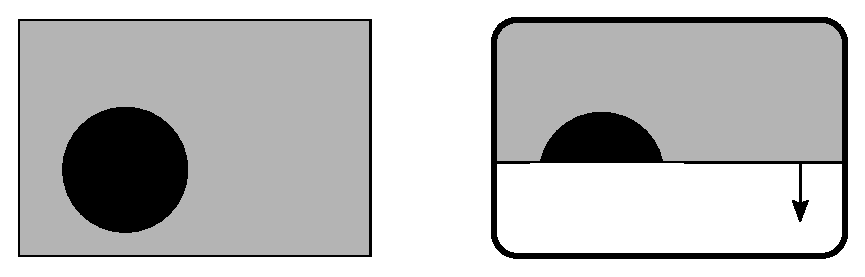
\includegraphics[width=\textwidth]{imgs/drawings/doublebuffer_before.eps}
\end{figure}
\par
In this example the CPU has finished writing the framebuffer (on the left) and the CRT (on the right) electron beam has started to scan it onto the screen. At this point in time the electron beam has scanned half the framebuffer and therefore the circle has been partially drawn on the screen.
\par
\begin{figure}[H]
\centering
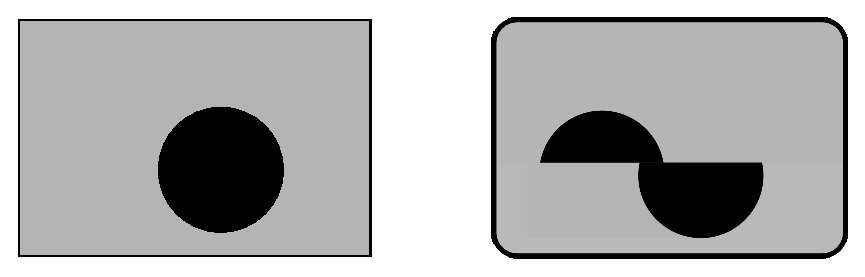
\includegraphics[width=\textwidth]{imgs/drawings/doublebuffer_after.eps}
\end{figure}
\par
But if the CPU is fast enough (faster than 70Hz), it can write the framebuffer again, before the scan is completed. This is what happened here. The next frame was drawn with the circle moved to the right. The electron beam did not know that and just kept on scanning the framebuffer. The result on screen is now a composite of two frames. It looks like two frames were torn and tapped back together. Hence the name "tearing".\\
\par
With two buffers (a.k.a double buffering) the CPU can start writing in the second framebuffer without messing with the framebuffer being scanned to the screen\footnote{Now the CPU speed is capped by the CRT refresh rate. Triple buffering can solve this at the price of frame latency.}. No more tearing!
















\section{Audio}
A PC came equipped with a beeper, commonly known as a "PC Speaker". This is a silver dollar sized buzzer capable of generating square wave via 2 levels of output.\\
\par
 \begin{figure}[H]
\centering
\includegraphics[width=\textwidth]{imgs/drawings/square_wave.pdf}
\caption{Two beeps of different frequencies generated via PC Speaker.}
\end{figure}

\par
 To this day, it is the first output device to be activated during the boot process. The purpose of this primitive loudspeaker is to signal hardware problems with beep codes. It was supposed to remain silent after a successful boot.\\
\par
\begin{tabularx}{\textwidth}{l l}
\textbf{Beep Code} & \textbf{Meaning}  \\ \hline
No Beeps                         & Short, Bad CPU/MB, Loose Peripherals \\ \hline
One Beep                         & Everything is normal\\ \hline
Two Beeps                        & POST/CMOS Error \\ \hline 
One Long Beep, One Short Beep    & Motherboard Problem \\ \hline
One Long Beep, Two Short Beeps   & Video Problem \\ \hline
One Long Beep, Three Short Beeps & Video Problem \\ \hline
Three Long Beeps                 & Keyboard Error \\ \hline
Repeated Long Beeps              & Memory Error \\ \hline
Continuous Hi-Lo Beeps           & CPU Overheating \\ \hline
\end{tabularx}\\
\bigskip
\par
Needless to say, square waves are not useful for anything pleasant to hear. Some people had started to see a market and they companies began manufacturing what were known as "sound cards". You could buy them separately and insert them into one of the ISA slots of the machine. These cards could be connected to real audio speakers via 3.5mm jack and tremendously improved sound capabilities. In 1991, Adlib, Creative, and Disney shared the market with four cards.\\
\par
\begin{itemize}
\item Adlib music card
\item SoundBlaster 1.0
\item SoundBlaster Pro
\item Disney Sound Source
\end{itemize}
\par
Even though adoption was increasing (Creative would go on to sell one million SoundBlaster cards in 1991), a vast majority of PCs had no sound card which once again presented a huge problem for game developers.


  \subsection{AdLib}
  AdLib was the first on the market. It was founded in 1988 by Martin Prevel, a former professor of music from Quebec. After an initial struggle to get game developers to use their card (the SDK was \$300), Adlib managed to convince Taito, Velocity, and Sierra On-Line to support their hardware. Sierra in particular did much to improve adoption with King's Quest IV selling close to 3 million copies. Soon after, all games supported the "music card".\\
  \par
   Equipped with a Yamaha YM3812, also known as the OPL2, the card can produce 9 channels of sound, each capable of simulating an instrument. Based on FM synthesizing, the channels were limited but allowed for pleasant music.\\
  \begin{figure}[H] 
    \centering 
    \scaledimage{.8}{hardware/adlib.png} 
    \caption{An Adlib sound card. Notice the YM3812 chip and the 8 bits ISA connector.}
  \end{figure}
   
\par
\bu{Trivia :} Canadian companies, and especially those from Quebec, were preponderant on the PC market in the early 90s due to their technological prowess. Ad Lib manufactured Sound Card, Matrox made a killing with its Millenium Graphic Card, and Watcom sold the best DOS C compiler\footnote{Watcom compiler was so good id would use it to compile Doom.}. ATI\footnote{History would repeat itself in the late 90s in the field of Graphic Cards: Nvidia Vs ATI} would later emerge as a major GPU innovator in the years 2000s.\\
  
  


  \subsection{Sound Blaster}
  The Sound Blaster 1.0 (code named "Killer Kard"), was released in 1989 by Creative. It was a smart product which was clearly targeting Adlib's dominant position. Not only was it equipped with the same OPL2 chip, providing 100\% compatibility with Adlib music playback, but it was also technologically superior with a DSP\footnote{An Intel MCS-51 market as a "Digital Sound Processor", not "Digital Signal Processor"}  allowing PCM playback (digitized sounds) at 8 bits per sample and up to 22.05Hz sampling rate. The card also came with a DA-15 port allowing connection of a joystick. Most importantly, the SoundBlaster was \$90 cheaper than the Adlib.\\ 
\par

\begin{figure}[H] 
  \centering 
  \fullimage{hardware/sb.png} 
  \caption{A SoundBlaster (v2). }
\end{figure}
\par
The above picture is the CT1350B model. Notice the OPL2 chip (labeled FM1312), the big CT1336 bus interface (labeled "CREATIVE") on the center left, the CT1351 DSP on the upper left and the 8 bits ISA bus connector.\\
\par
  \bu{Trivia :} The numerous qualities of the card over the Adlib made the Sound Blaster the de-facto standard shortly after its release and eventually brought Adlib to bankruptcy\footnote{The reign of the Sound Blaster came to an end with Windows 95, which standardized the programming interface at application level and eliminated the importance of compatibility with Sound Blaster}.





  \subsection{Sound Blaster Pro}
The Sound Blaster Pro had all the capabilities of a Sound Blaster 1.0 but added support for stereo 22.05 kHz playback and 44.1 kHz in mono. It also added a "mixer" to blend audio sources from mic, line in, and, CD and chose the attenuation level of left and right outputs. Stereo was achieved with a pair of YM3812 chips (one for each audio channel).\\\label{sbmixerpage}
\begin{figure}[H] 
  \centering 
  \fullimage{hardware/sbpro.png} 
  \caption{A Sound Blaster Pro card.}
\end{figure}
The model above is a CT1330A. Notice the double FM1312 chip in the center. The two big chips in the upper left are the DSP (CT1341) and the Mixer. Below, labeled "Creative" is the big CT1316 bus interface.\\
\par
\bu{Trivia :} The card appears to have a 16 bits ISA bus connector (check the difference with a Sound Blaster 1.0). However it does not have 'fingers' for data transfer on the higher "AT" portion of the bus connector. It uses the 16-bit extension to the ISA bus to provide the user with an additional choice for an IRQ (10) and DMA (0)m channel only found on the 16-bit portion of the edge connector.\\
\par
\bu{Trivia :} Notice on the very left of the card in black an IDE Data interface to connect a CD-ROM. That was the only way to connect a CD-ROM to a PC back then.


  \subsection{Disney Sound Source}
  Debuting in 1990, Disney sold a marvelous piece of audio hardware. Plugged into the printer port (parallel port) of the PC, a 8 bits DAC based on the "Covox Speech Thing" was connected to a speaker box. It was incredibly easy to setup, simple to program (it could only play one type of PCM and had no FM synthesizer) and very cheap compared to the other audio solutions (\$14). It would have made programmers and customers happy if it was not for a serious issue due to the bandwidth of the port (150 kbit/s) which limited the PCM sampling rate to 7000Hz.  This was still enough to produce pleasant sounds but fell short when compared to the 22Hz or even 44Khz of a Sound Blaster Pro.
  \par
  \begin{figure}[H] 
    \centering 
    \fullimage{hardware/ss.png} 
    \caption{The speaker box (DAC not shown).}
  \end{figure}








\section{Inputs}
At a time before the ubiquitous USB, inputs were a mess with no less than four ports, all programmed differently.\\

The parallel port (DB-25) was on every computer and usually used to connect matrix printers (loud thing that printed with needles). The parallel port was multipurpose and the Disney Sound Source could be plugged into it.\\
\par
 \begin{figure}[H]
\centering
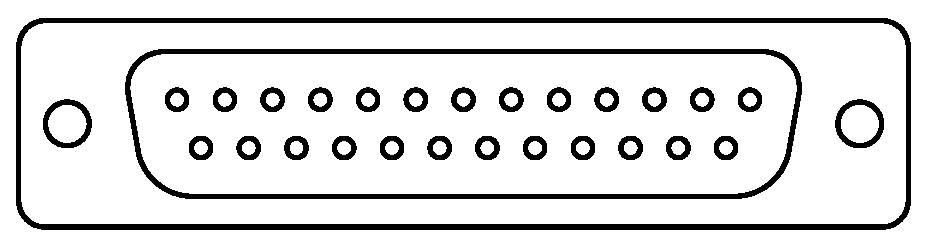
\includegraphics[width=0.3\textwidth]{imgs/drawings/ports/DB-25_parallel_port.eps}
\caption{Parallel Port}
\label{fig:parallelPort}
\end{figure}


The serial port (DE9) was used to connect the mouse:
 \begin{figure}[H]
\centering
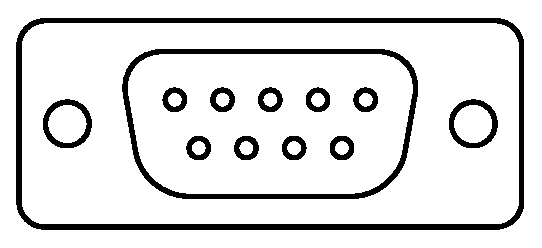
\includegraphics[width=0.15\textwidth]{imgs/drawings/ports/DE9_serial_port.eps}
\caption{Serial Port}
\label{fig:serialPort}
\end{figure}

The PS/2 port was used to connect a keyboard:
 \begin{figure}[H]
\centering
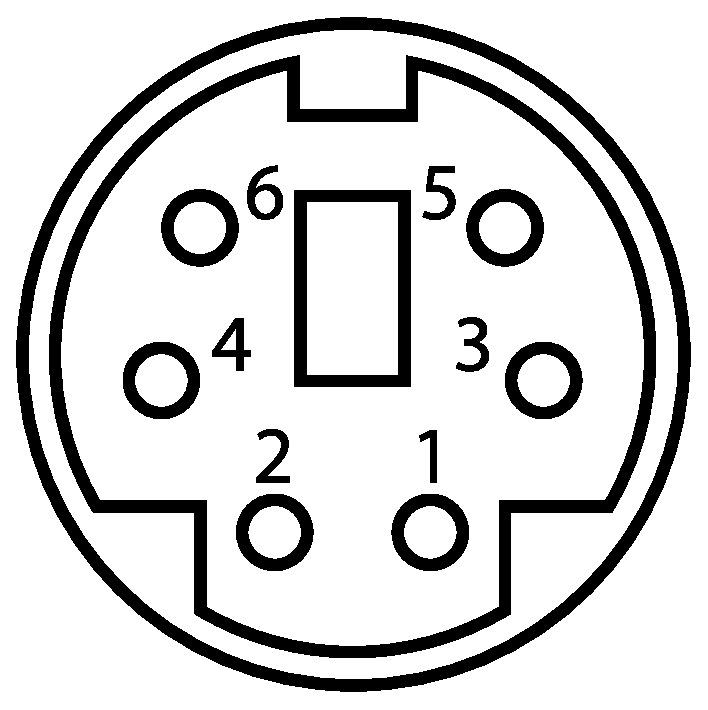
\includegraphics[width=0.07\textwidth]{imgs/drawings/ports/MiniDIN-6_PS2.eps}
\caption{PS/2 Port}
\label{fig:ps2Port}
\end{figure}


Finally, the sound card connected via the ISA bus provided a new port: a Game Port (DA-15) allowing for connection to a joystick:
 \begin{figure}[H]
\centering
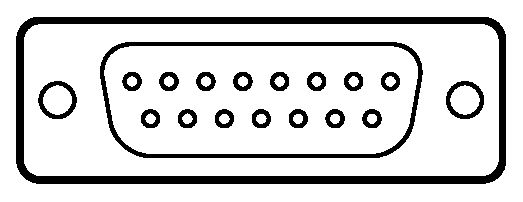
\includegraphics[width=0.19\textwidth]{imgs/drawings/ports/DA-15_GamePort.eps}
\caption{Game Port}
\label{fig:gamePort}
\end{figure}

\bu{Trivia :} The CRT monitor was connected to the VGA card via a DE15 port. More than 20 years later manufacturers are still trying to get ride of the "VGA port" as it is now commmonly called.
 \begin{figure}[H]
\centering
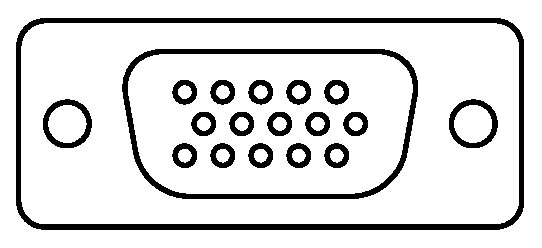
\includegraphics[width=0.14\textwidth]{imgs/drawings/DE15_VGA.eps}
\caption{VGA Port}
\label{fig:ps2Port}
\end{figure}


\section{Bus}
Although developers had no control over them, it is still worth mentioning how these components were connected to each others.\\ 
\par

The ISA\footnote{Industry Standard Architecture} bus connectes the CPU to all devices, including RAM. It was already 10 years old in 1991 but still used universally in every PC shipping. The data path to the RAM is either 16 bits wide for 286 and 386SX or 32 bits on 386DX based machines. It runs at the same frequency as the CPU.\\
\par
The rest of the bus connecting to everything that is not the RAM can be of two kinds:
\begin{itemize}
\item 8-bit wide at 4.77 MHz  for 19.1 Mbit/s
\item 16-bit wide at 8.33MHz for 66.7 Mbit/s\footnote{https://en.wikipedia.org/wiki/List\_of\_device\_bit\_rates}.
\end{itemize}
Of course it is also backward compatible and an 8 bits ISA card can be plugged into a 16 bits ISA bus.\\
\par
\begin{figure}[H]
\centering
      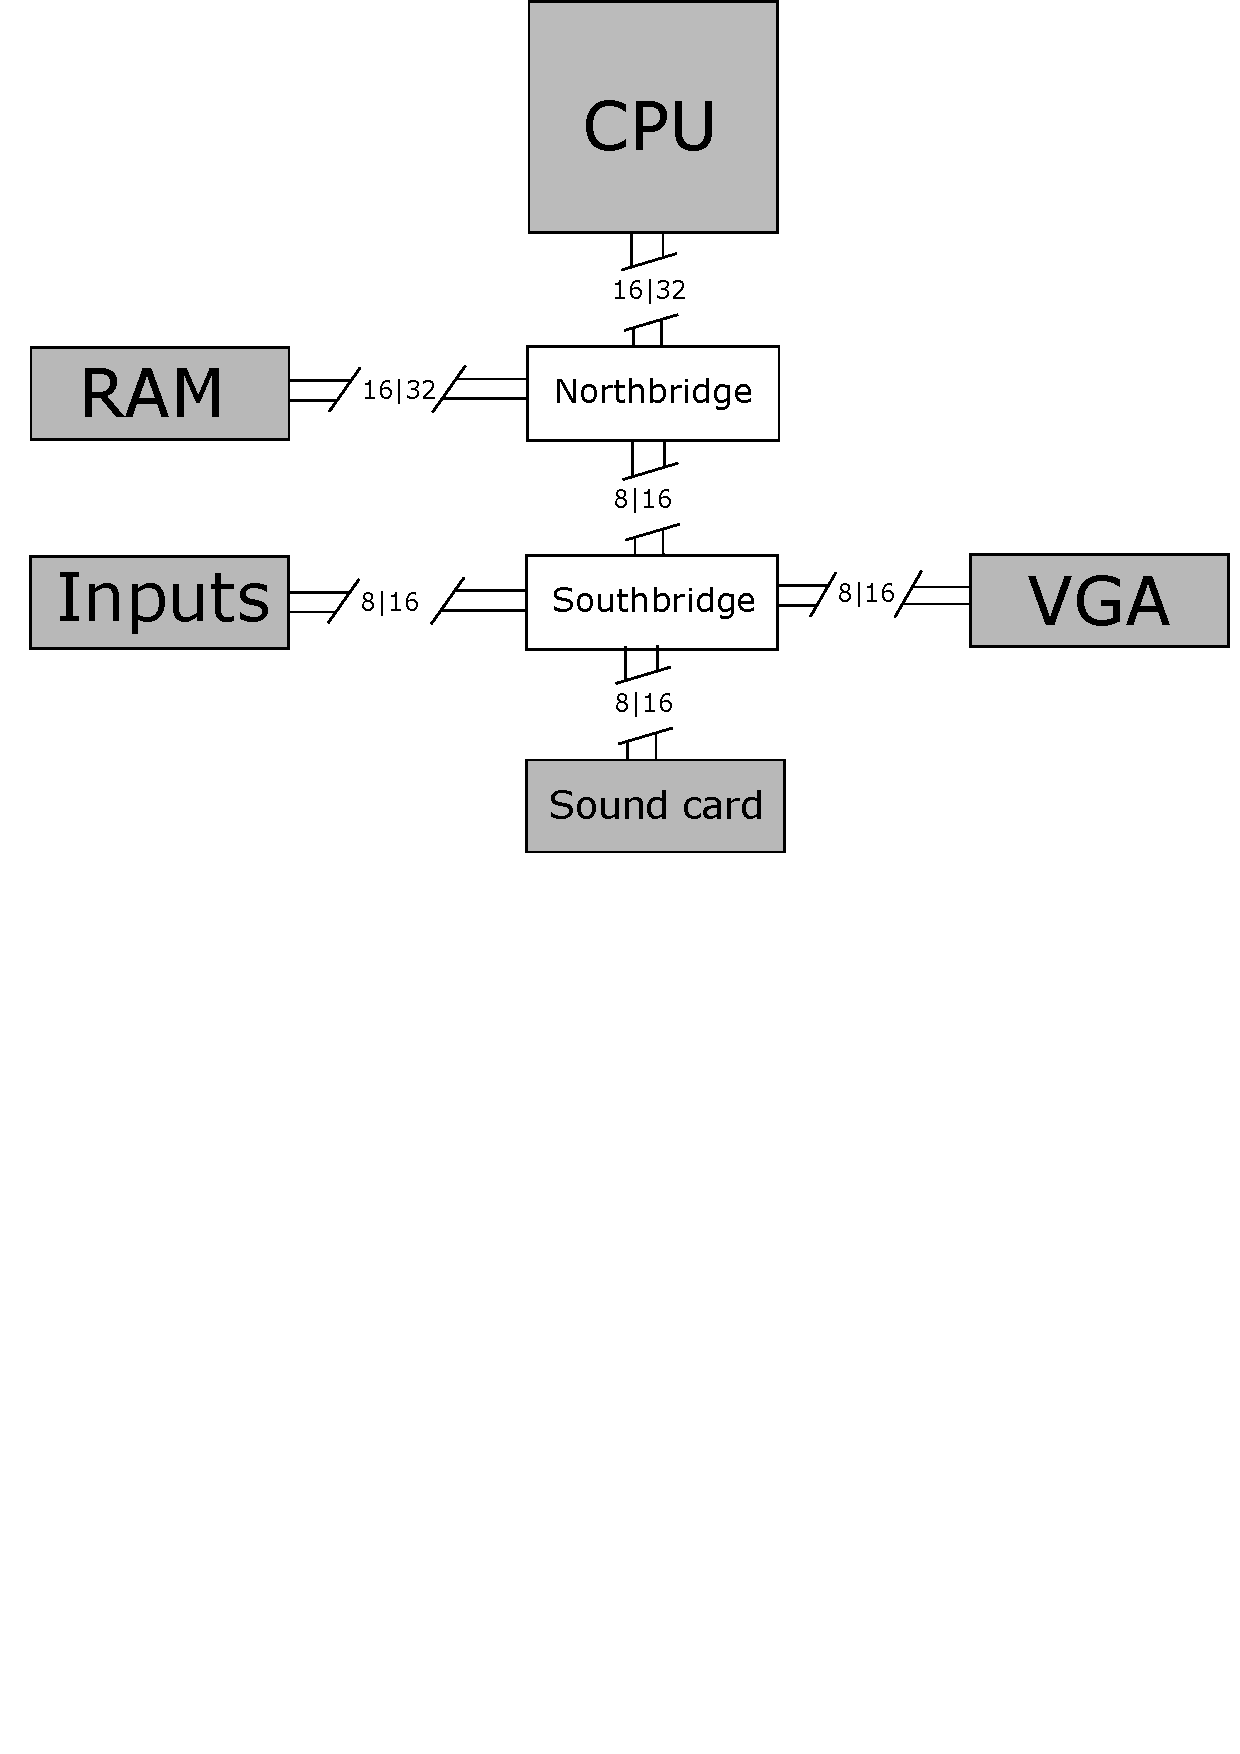
\includegraphics[width=\textwidth]{imgs/drawings/bus.pdf}
\end{figure}
\par
\bu{Trivia :} On ISA all devices are connected to the bus at all time and listen on the bus address lane. Each device features an "address decoder" to detect if it should reply to a bus request. This is how the VGA RAM is "mapped" in RAM. The VGA card "address decoder"  filters out everything that is not within \cw{A0000h} and \cw{AFFFFh}. Accordingly the RAM disregard any request that is within the range [\cw{A0000h} - \cw{AFFFFh}].\\
\par
 \begin{figure}[H]
\centering
\includegraphics[width=\textwidth]{imgs/drawings/isa.pdf}
\end{figure}

\par
 In practice, due to packet overhead and interrupts, the effective bandwidth of the bus is divided by two. As a result, a PC equipped with an 8-bits ISA VGA card can push 19.1Mbits/s/2 = 1.5MB/s. In Mode 13h, since a frame is 320x200 = 64,000 bytes, the theoretical maximum framerate with a CPU taking 0ms to render a frame is 1,500,000 / 64,000 = 23 frames per seconds.\\
 \par
 On a 16 bits VGA card, 33,400,000 bits per seconds gives 33,400,000/8/64000 = 65 frames per seconds.\\
 \par
 If you factor in other things which had to transit on the bus such as palette, keyboard interrupt, mouse inputs, and music/sounds (at 23kHz sampling a digitized sound effect consumes 23,000/70 = 328 bytes per frame) it is easy to understand how important it was to limit data transfer and why few software of the era could max out the VGA's 70 frame per seconds\footnote{Specialized demos could reach 70 fps on VGA by careful management of unchanged regions or using planar writes for the 4x speedup.}.


\section{Summary}
To say a PC was difficult to program for games would be an understatement. It was nightmare. The CPU was good at doing the wrong thing, the best graphic interface allowed neither double buffering nor square pixels, the memory model only allowed 1 standard MB with address composed of two separate 16 bits registers and the \cw{near}/\cw{far} pointers forbade using standard C. Last but not least, the default sound system could only produce square waves and the people who did have a sound card installed could have any of the three major brands.\\
\par
Yet despite all these unfavorable conditions, teams of developers gathered to tame the beast and unleash its power to gamers. One of them called themselves id Software\footnote{They originally called themselves Ideas From the Deep but they decided to shortened it to simply id, which stands for "in demand," and is pronounced as in "did" or "kid." The name also had another meaning which is referring to id, one of the three parts (the other two being ego and super-ego) of the brain that behaves by the pleasure principle.}.
\end{document}




